% Gói & Cấu hình tài liệu
\documentclass[en]{IPLeiriaThesis}

% Cấu hình listings để in code học thuật đơn giản, không màu mè
\usepackage{listings}
\usepackage{enumitem}
\usepackage{tikz}
\usepackage{booktabs}
\usepackage{tabularx}
\usepackage{multirow}
\usepackage{longtable}

\lstset{
    basicstyle=\ttfamily\footnotesize,
    keywordstyle=\bfseries\color{blue!70!black},
    commentstyle=\itshape\color{gray!70!black},
    stringstyle=\color{green!50!black},
    numbers=left,
    numberstyle=\tiny\color{gray},
    stepnumber=1,
    numbersep=6pt,
    backgroundcolor=\color{gray!3},
    showspaces=false,
    showstringspaces=false,
    showtabs=false,
    frame=single,
    rulecolor=\color{gray!30},
    tabsize=4,
    captionpos=b,
    breaklines=true,
    breakatwhitespace=false
}

\lstdefinestyle{terminal}{
    basicstyle=\ttfamily\footnotesize,
    backgroundcolor=\color{gray!5},
    frame=single,
    rulecolor=\color{gray!30},
    numbers=none,
    breaklines=true
}

% Tài liệu về các tham số (Tiêu đề đề tài, nhóm tác giả, v.v.)
% Đảm bảo định nghĩa lệnh cho thành viên thứ 6 và thứ 7 ngay cả khi dùng file cls gốc
\makeatletter
\providecommand{\sixthauthor}[1]{\gdef\sixthauthorname{#1}}
\providecommand{\seventhauthor}[1]{\gdef\seventhauthorname{#1}}
\makeatother

% Authors (Nhóm 2 - Lớp M26CQ02)
\firstauthor{Hoàng Anh Tuấn - B26CHHT102}
\secondauthor{Đào Duy Thông - B26CHHT095}
\thirdauthor{Nguyễn Hoàng Mạnh Dũng - B26CHHT026}
\fourthauthor{Hồ Quang Anh - B26CHHT005}
\fifthauthor{Nguyễn Thị Ngọc Bích - B26CHHT010}
\sixthauthor{Nguyễn Ngọc Quang - B26CHHT086}
\seventhauthor{Hoàng Minh Dũng - B26CHHT027}

% Supervisor (Mandatory)
\supervisor{TS. Phan Thị Hà}
\supervisormail{hapt@ptit.edu.vn}

% Title (Mandatory)
\title{BÁO CÁO BÀI TẬP LỚN CÁC HỆ THỐNG CƠ SỞ DỮ LIỆU}

% Subtitle (Mandatory)
\subtitle{ĐỀ TÀI 13: XÂY DỰNG HỆ CƠ SỞ DỮ LIỆU QUẢN LÝ MỘT GIẢI BÓNG ĐÁ CHUYÊN NGHIỆP}

% University (Mandatory)
\university{Học viện Công nghệ Bưu chính Viễn thông}

% Department (Mandatory)
\department{Khoa Sau Đại học}

% Degree (Mandatory)
\degree{Lớp: M26CQ02 (HTTT) -- Nhóm 2}

% Course (Optional)
\course{Học phần: Các hệ thống Cơ sở dữ liệu}

% Local & Date (Mandatory)
\date{Hà Nội, \number\year}


% Tạo và Tải Thuật ngữ & Từ viết tắt
\makeglossaries
\loadglsentries{Matter/04-Glossary}
\loadglsentries[\acronymtype]{Matter/05-Acronyms}

\begin{document}

% Nội dung của trang bìa và trang lót
\ifthenelse{\equal{\getLanguage}{portuguese}}{%
    \pdfbookmark[0]{Capa}{capa} % Add entry to PDF bookmarks group
    \pdfbookmark[1]{Frontispício}{frontispício} % Add entry to PDF
}{%
    \pdfbookmark[0]{Front Matter}{frontmatter} % Add entry to PDF bookmarks group
    \pdfbookmark[1]{Cover}{cover} % Add entry to PDF
}

% Add background picture
\newcommand\BackgroundPicCover{%
    \put(0,0){%
    \parbox[b][\paperheight]{\paperwidth}{%
    \vfill
    \centering
    
\includegraphics[width=\paperwidth,height=\paperheight,keepaspectratio]{Figures/Theme/Cover-BG.pdf}%
    \vfill
}}}
\AddToShipoutPictureBG*{\BackgroundPicCover}

\newgeometry{margin=1.98cm, top=2.15cm, bottom=1.47cm}
\begin{titlepage}
    \latofont % Switch to Lato font for the title page
    \color{white} % Define the color to use within this page
    \vspace*{\baselineskip} % White space at the top of the page

    \begin{figure}
        
\includegraphics[width=0.75\linewidth]{Figures/Theme/ptit_logo_red-removebg.png}
    \end{figure}

    \vspace{5.5\baselineskip}

    % Title
	\noindent
    \makebox[\textwidth][l]{%
        \parbox{\dimexpr\textwidth-2.5cm\relax}{
            \setstretch{1.03}
            \raggedright\bfseries\fontsize{20}{26}\selectfont\thetitle
        }
    }

    \vspace{0.8\baselineskip}

    % Subtitle
    \noindent
    \makebox[\textwidth][l]{%
        \parbox{\dimexpr\textwidth-7cm\relax}{
            \setstretch{1.03}
            \raggedright\fontsize{14}{19}\selectfont\subname
        }
    }

    \vspace{25pt}  

    % Authors (Nhóm 7 thành viên)
    {\noindent\bfseries\fontsize{11}{14}\selectfont\firstauthorname}

    \ifdefined\secondauthorname
        \vspace{4pt}
        {\noindent\bfseries\fontsize{11}{14}\selectfont\secondauthorname}
	\fi

    \ifdefined\thirdauthorname
        \vspace{4pt}
        {\noindent\bfseries\fontsize{11}{14}\selectfont\thirdauthorname}
	\fi

    \ifdefined\fourthauthorname
        \vspace{4pt}
        {\noindent\bfseries\fontsize{11}{14}\selectfont\fourthauthorname}
	\fi

    \ifdefined\fifthauthorname
        \vspace{4pt}
        {\noindent\bfseries\fontsize{11}{14}\selectfont\fifthauthorname}
	\fi
 
    \ifdefined\sixthauthorname
        \vspace{4pt}
        {\noindent\bfseries\fontsize{11}{14}\selectfont\sixthauthorname}
	\fi

    \ifdefined\seventhauthorname
        \vspace{4pt}
        {\noindent\bfseries\fontsize{11}{14}\selectfont\seventhauthorname}
	\fi
 
	\vfill

    % School
	% {\noindent\fontsize{10}{12}\selectfont\schoolname}
	
    % Department
	{\noindent\fontsize{10}{12}\selectfont\departmentname}

    % Degree
	% {\noindent\fontsize{10}{12}\selectfont\degname}

    % Course
    \ifdefined\coursename
        {\noindent\fontsize{10}{12}\selectfont\coursename}
	\fi

    \vspace{105pt}

    % Local & Date
	{\noindent\fontsize{10}{12}\selectfont\thedate}

    \vspace{68pt}
\end{titlepage}
\restoregeometry\blankpage
\ifthenelse{\equal{\getLanguage}{portuguese}}{%
    \pdfbookmark[1]{Primeira Página}{primeirapagina} % Add entry to PDF
}{%
    \pdfbookmark[1]{Front Page}{frontpage} % Add entry to PDF
}

% Add background picture
\newcommand\BackgroundPicFrontPage{%
    \put(0,0){%
    \parbox[b][\paperheight]{\paperwidth}{%
    \vfill
    \centering
    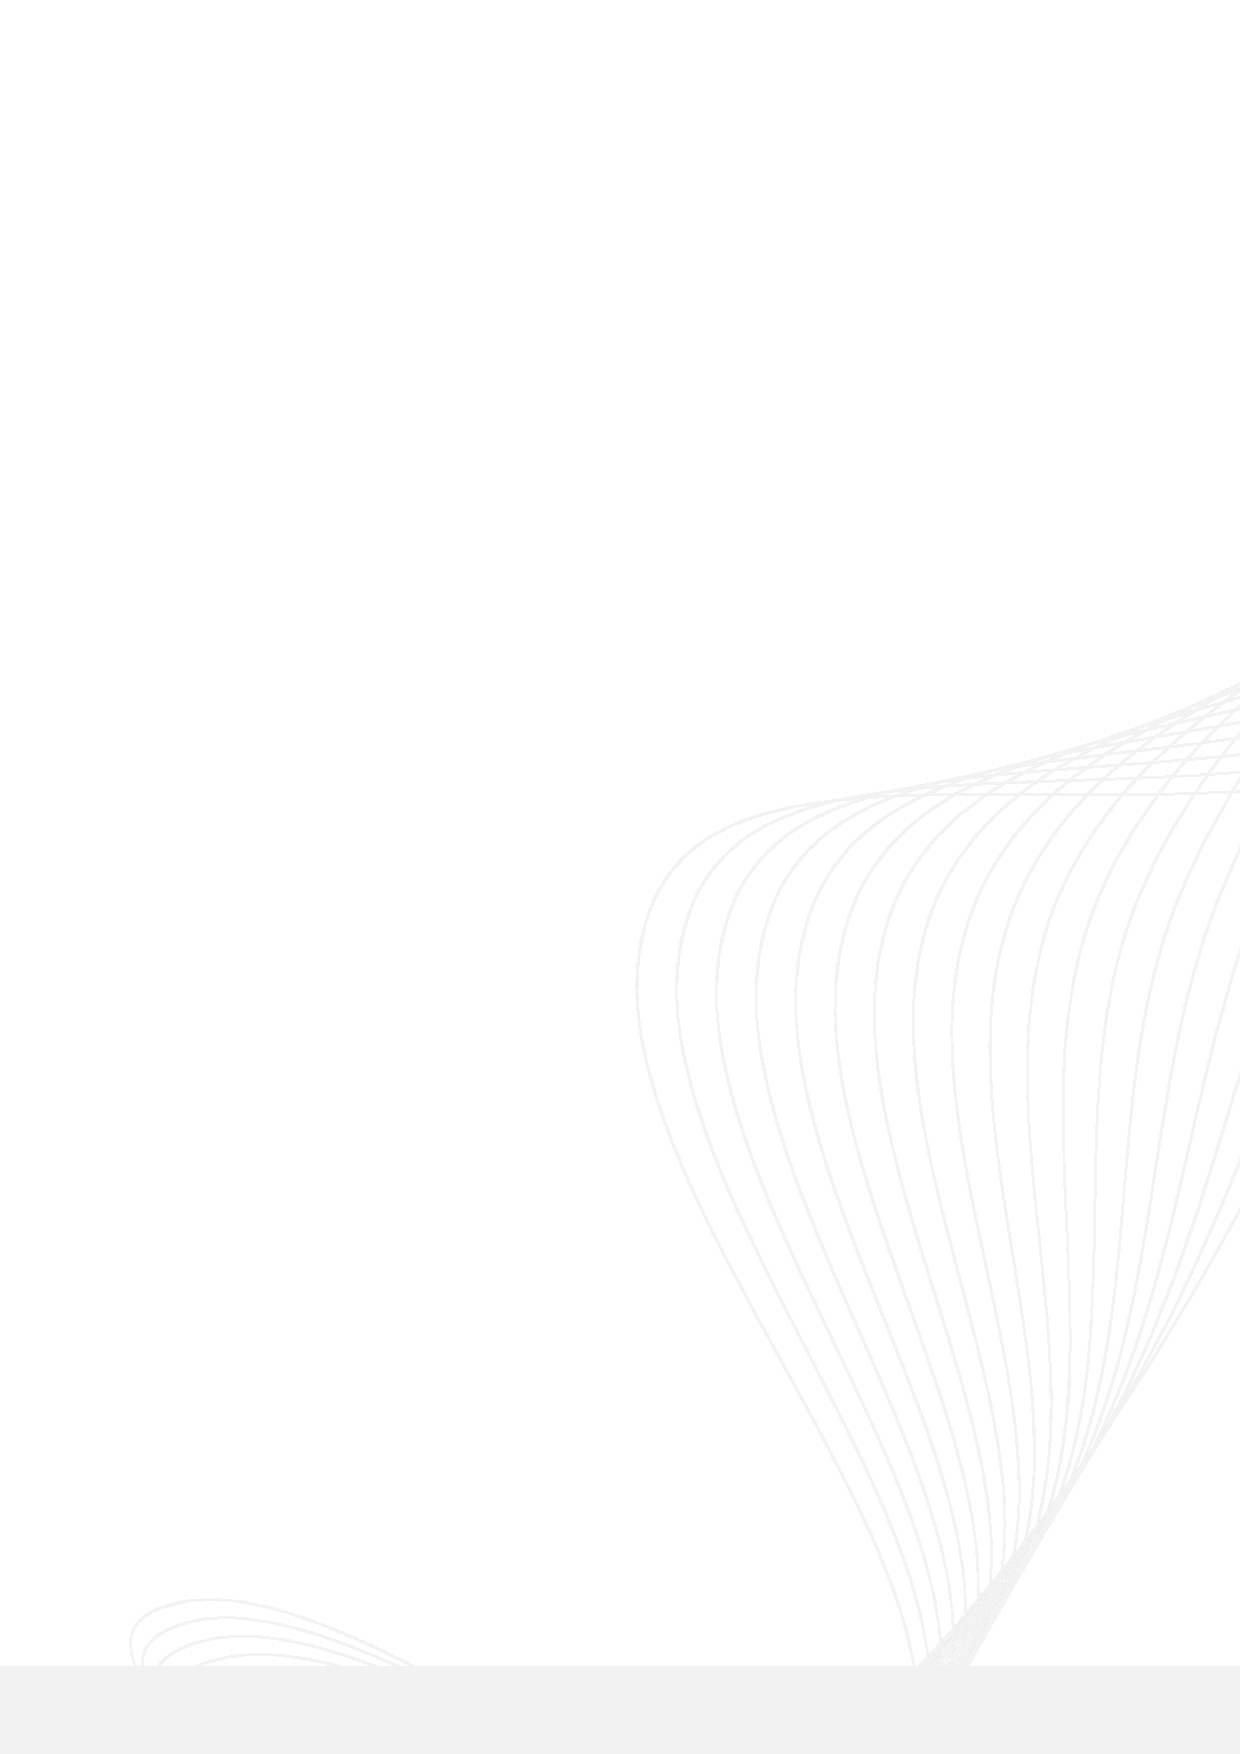
\includegraphics[width=\paperwidth,height=\paperheight,keepaspectratio]{Figures/Theme/Front-Page-BG.pdf}%
    \vfill
}}}
\AddToShipoutPictureBG*{\BackgroundPicFrontPage}

\newgeometry{margin=1.98cm, top=2.15cm, bottom=1.47cm}
\begin{titlepage}
    \latofont % Switch to Lato font for the title page
    \color{frontpagedark} % Define the color to use within this page
    \vspace*{\baselineskip} % White space at the top of the page

    \begin{figure}
        
\includegraphics[width=0.75\linewidth]{Figures/Theme/ptit_logo_red-removebg-gray.png}
    \end{figure}

    \vspace{3.5\baselineskip}

    % Title
	\noindent
    \makebox[\textwidth][l]{%
        \parbox{\dimexpr\textwidth-2.5cm\relax}{
            \setstretch{1.03}
            \raggedright\bfseries\fontsize{20}{26}\selectfont\thetitle
        }
    }

    \vspace{0.8\baselineskip}

    % Subtitle
    \noindent
    \makebox[\textwidth][l]{%
        %\fbox{%
            \parbox{\dimexpr\textwidth-7cm\relax}{
                \setstretch{1.03}
                \raggedright\fontsize{14}{19}\selectfont\subname
            }
        %}
    }

    \vspace{25pt}

    % Authors (Nhóm 7 thành viên)
    {\noindent\bfseries\fontsize{11}{14}\selectfont\firstauthorname}

    \ifdefined\secondauthorname
        \vspace{4pt}
        {\noindent\bfseries\fontsize{11}{14}\selectfont\secondauthorname}
	\fi

    \ifdefined\thirdauthorname
        \vspace{4pt}
        {\noindent\bfseries\fontsize{11}{14}\selectfont\thirdauthorname}
	\fi

    \ifdefined\fourthauthorname
        \vspace{4pt}
        {\noindent\bfseries\fontsize{11}{14}\selectfont\fourthauthorname}
	\fi

    \ifdefined\fifthauthorname
        \vspace{4pt}
        {\noindent\bfseries\fontsize{11}{14}\selectfont\fifthauthorname}
	\fi

    \ifdefined\sixthauthorname
        \vspace{4pt}
        {\noindent\bfseries\fontsize{11}{14}\selectfont\sixthauthorname}
	\fi

    \ifdefined\seventhauthorname
        \vspace{4pt}
        {\noindent\bfseries\fontsize{11}{14}\selectfont\seventhauthorname}
	\fi

    \vspace{40pt}    

    {
    \noindent
    \latofont
    \fontsize{10}{12}\selectfont
    \renewcommand{\arraystretch}{0.1}
    \hspace*{-2.5pt}\begin{tabular}{@{}r@{\hspace{5pt}}>{\raggedright\arraybackslash}m{6cm}@{}}
        \textbf{Giảng viên hướng dẫn:} & \supname \\ [-.7ex]
       % & \setstretch{0.9}{\fontsize{8}{10}\selectfont\itshape \suptitle} \\ [2ex]
        
        \ifdefined\cosupname
            \textbf{Co-supervisor:} & \cosupname \\ [-.7ex]
            & \setstretch{0.9}{\fontsize{8}{10}\selectfont\itshape \cosuptitle} \\ [.5ex]
        \fi

        \ifdefined\seccosupname        
            & \seccosupname \\ [-.7ex]
            & \setstretch{0.9}{\fontsize{8}{10}\selectfont\itshape \seccosuptitle} \\
        \fi
    \end{tabular}
    }
    
    \vfill
	
    % School
	% {\noindent\fontsize{10}{12}\selectfont\schoolname}
	
    % Department
	{\noindent\fontsize{10}{12}\selectfont\departmentname}

    % Degree
	% {\noindent\fontsize{10}{12}\selectfont\degname}

    % Course
    \ifdefined\coursename
        {\noindent\fontsize{10}{12}\selectfont\coursename}
	\fi

    \vspace{75pt}

    % Local & Date
	{\noindent\fontsize{10}{12}\selectfont\thedate}

    \vspace{68pt}
\end{titlepage}
\restoregeometry

% Đánh số la mã cho phần đầu
\pagenumbering{roman}

% Lời cảm ơn
\thispagestyle{plain}

\ifthenelse{\equal{\getLanguage}{portuguese}}{%
    \pdfbookmark[1]{Agradecimentos}{agradecimentos}
    \chapter*{Agradecimentos}
}{%
    \pdfbookmark[1]{Acknowledgements}{acknowledgements}
    \chapter*{Lời cảm ơn}
}

\begin{flushleft}
Nhóm sinh viên chúng em xin gửi lời cảm ơn chân thành và sâu sắc nhất tới quý Thầy, Cô Học viện Công nghệ Bưu chính Viễn thông, những người đã tận tâm giảng dạy, truyền đạt những kiến thức nền tảng và chuyên sâu quý báu trong suốt quá trình học tập tại học viện.

\vspace{1em}

Đặc biệt, nhóm xin bày tỏ lòng biết ơn sâu sắc tới Giảng viên hướng dẫn môn học \textbf{Các hệ thống Cơ sở dữ liệu} - người đã trực tiếp định hướng phương pháp tiếp cận, cung cấp tài liệu giảng dạy và tận tình hướng dẫn nhóm trong suốt quá trình thực hiện bài tập lớn, từ khâu khảo sát nghiệp vụ thế giới thực, thiết kế mô hình E-R, chuẩn hóa BCNF, xây dựng hệ CSDL, phân tích thiết kế CSDL phân tán cho đến hoàn thiện ứng dụng phần mềm.

\vspace{1em}

Mặc dù nhóm đã nỗ lực hết mình để hoàn thiện báo cáo và hệ thống một cách chỉn chu nhất, song do giới hạn về thời gian và kiến thức thực tế, báo cáo khó tránh khỏi những thiếu sót nhất định. Nhóm rất mong nhận được những ý kiến đóng góp quý báu từ quý Thầy/Cô để đề tài được hoàn thiện hơn nữa.

\vspace{1.5em}

\begin{flushright}
\textbf{Nhóm sinh viên thực hiện}\\
\textit{Hà Nội, năm 2026}
\end{flushright}
\end{flushleft}


% Phần tóm tắt
\thispagestyle{plain}

\ifthenelse{\equal{\getLanguage}{portuguese}}{%
    \pdfbookmark[1]{Resumo}{resumo}
    \chapter*{Resumo}
}{%
    \pdfbookmark[1]{Abstract}{abstract}
    \chapter*{Tóm tắt báo cáo}
}

Báo cáo Bài tập lớn môn \textbf{Các hệ thống Cơ sở dữ liệu} thực hiện nghiên cứu, phân tích và triển khai toàn diện \textbf{Hệ cơ sở dữ liệu quản lý một giải bóng đá chuyên nghiệp} (Đề tài 13). Hệ thống được xây dựng nhằm đáp ứng các yêu cầu nghiệp vụ thực tế của một mùa giải bóng đá: quản lý câu lạc bộ, cầu thủ, sân vận động, đội ngũ trọng tài, hợp đồng thi đấu và cho mượn cầu thủ; thiết lập lịch thi đấu vòng tròn hai lượt ($10$ vòng, $30$ trận); đăng ký đội hình tối đa 18 cầu thủ mỗi trận; theo dõi chi tiết các sự kiện diễn biến trên sân (bàn thắng, thẻ phạt) và tính toán bảng xếp hạng tự động. 

Nội dung báo cáo bao gồm: (1) Phân tích yêu cầu và thiết kế Lược đồ thực thể liên kết chi tiết (E-R); (2) Ánh xạ sang Lược đồ quan hệ và chứng minh giải tích toàn bộ $11$ quan hệ đạt \textbf{Dạng chuẩn BCNF (Boyce-Codd Normal Form)}; (3) Cài đặt CSDL trên hệ quản trị với đầy đủ ràng buộc toàn vẹn, ít nhất $5$ Transaction và $5$ Trigger nghiệp vụ phức tạp; (4) Phân tích và thiết kế \textbf{Cơ sở dữ liệu phân tán (CSDLPT)} theo mô hình đa chi nhánh gồm phân mảnh ngang, phân mảnh dọc, phân mảnh dẫn xuất và nhân bản dữ liệu; (5) Xây dựng ứng dụng giao diện trực quan kết nối CSDL phục vụ tra cứu, cập nhật dữ liệu, tính lương trọng tài và thống kê doanh thu bán vé.

\vspace{1cm}

\noindent\textbf{Từ khóa:} Cơ sở dữ liệu, Lược đồ E-R, Chuẩn hóa BCNF, CSDL Phân tán, Phân mảnh dữ liệu, Quản lý giải bóng đá, Trigger, Transaction.


\renewcommand{\contentsname}{Mục lục}
\renewcommand{\listfigurename}{Danh sách hình vẽ}
\renewcommand{\listtablename}{Danh sách bảng biểu}

% Mục lục, hình ảnh và bảng biểu
\tableofcontents
\listoffigures
\listoftables

% Tùy chỉnh các tiêu đề
\renewcommand{\glossaryname}{Chú giải thuật ngữ}
\renewcommand{\acronymname}{Danh mục từ viết tắt}
\renewcommand{\tablename}{Bảng}
\renewcommand{\bibname}{Tài liệu tham khảo}

% Thuật ngữ và Từ viết tắt
\printglossary
\printglossary[type=\acronymtype]

% Đánh số Ả Rập cho phần nội dung chính
\pagenumbering{arabic}

% Nội dung các chương Báo cáo BTL Các hệ thống CSDL
\chapter{KHẢO SÁT BÀI TOÁN VÀ THIẾT KẾ LƯỢC ĐỒ THỰC THỂ LIÊN KẾT (E-R)}

\section{Mô tả bài toán và Khảo sát yêu cầu}

\subsection{Bối cảnh và Quy mô hệ thống}
Trong khuôn khổ bài tập lớn môn học \textit{Các hệ thống Cơ sở dữ liệu}, đề tài đặt ra yêu cầu xây dựng một hệ thống cơ sở dữ liệu (CSDL) quản lý toàn diện một giải bóng đá chuyên nghiệp cấp quốc gia trong một mùa giải. Hệ thống phải đảm bảo theo dõi chặt chẽ tất cả các khía cạnh nghiệp vụ từ thông tin các câu lạc bộ, cầu thủ, sân vận động, đội ngũ trọng tài, cho đến công tác lập lịch thi đấu vòng tròn hai lượt, đăng ký đội hình trước trận đấu, diễn biến chi tiết sự kiện trên sân (bàn thắng, thẻ phạt) và tính toán bảng xếp hạng tự động.

Theo yêu cầu của đề bài, các thông số cơ bản của mùa giải được xác định như sau:
\begin{itemize}
    \item \textbf{Số lượng đội bóng tham gia}: Chọn $N = 6$ đội bóng (thỏa mãn yêu cầu số chẵn tối thiểu $\ge 6$).
    \item \textbf{Thể thức thi đấu}: Vòng tròn 2 lượt (lượt đi sân nhà, lượt về sân khách). Với 6 đội, số vòng đấu là $2 \times (6 - 1) = 10$ vòng đấu. Mỗi vòng đấu diễn ra 3 trận đấu cùng một thời điểm giữa 3 cặp đấu.
    \item \textbf{Tổng số trận đấu trong cả mùa giải}: $10 \text{ vòng} \times 3 \text{ trận/vòng} = 30 \text{ trận đấu}$. Toàn bộ lịch thi đấu và kết quả của 30 trận này phải được nhập đầy đủ vào hệ thống.
\end{itemize}

\subsection{Các quy tắc nghiệp vụ cốt lõi}
Hệ thống phải tuân thủ nghiêm ngặt các ràng buộc nghiệp vụ thế giới thực được nêu trong đề cương bài toán:
\begin{enumerate}
    \item \textbf{Ràng buộc về Đội bóng, Sân nhà và Trang phục}:
    \begin{itemize}
        \item Mỗi đội bóng sở hữu đúng 1 sân nhà cố định. Tuy nhiên, một sân vận động có thể là sân nhà của một hoặc nhiều đội bóng khác nhau.
        \item Mỗi đội bóng phải đăng ký tối thiểu từ 2 màu áo thi đấu trở lên (ví dụ: áo sân nhà, áo sân khách, áo phụ).
        \item Một đội bóng được đăng ký tối đa 30 cầu thủ trong danh sách thi đấu mùa giải.
    \end{itemize}
    \item \textbf{Ràng buộc về Cầu thủ, Hợp đồng và Số áo}:
    \begin{itemize}
        \item Mỗi cầu thủ ký hợp đồng chuyên nghiệp với một đội bóng chủ quản. Cầu thủ có thể được đem cho một đội bóng khác mượn trong một khoảng thời gian nhất định.
        \item Tại mỗi thời điểm, mỗi cầu thủ chỉ được phép thi đấu cho duy nhất một đội bóng.
        \item Số áo thi đấu của cầu thủ bắt buộc phải nằm trong miền giá trị từ $1$ đến $35$.
        \item Trong cùng một đội bóng, các cầu thủ không được phép trùng số áo nhau; cầu thủ ở hai đội bóng khác nhau hoàn toàn có thể mang cùng số áo.
    \end{itemize}
    \item \textbf{Ràng buộc về Trọng tài và Phân công điều khiển}:
    \begin{itemize}
        \item Mỗi trận đấu bắt buộc phải có đủ tổ gồm 4 trọng tài làm nhiệm vụ: 1 trọng tài chính, 2 trọng tài biên và 1 trọng tài bàn.
        \item Trong cùng một vòng đấu, một trọng tài chỉ được phép điều khiển tối đa 1 trận đấu.
    \end{itemize}
    \item \textbf{Ràng buộc về Đăng ký thi đấu và Khớp kết quả trận}:
    \begin{itemize}
        \item Trận đấu có hai trạng thái: \textit{Chưa diễn ra} (lịch thi đấu tương lai) hoặc \textit{Đã kết thúc}. Nếu trận đấu đã kết thúc, ngày giờ thi đấu không được vượt quá thời gian hiện tại.
        \item Trong mỗi trận đấu, mỗi đội bóng chỉ được đăng ký tối đa 18 cầu thủ (gồm đội hình xuất phát và danh sách dự bị).
        \item Danh sách các sự kiện bàn thắng, thẻ vàng, thẻ đỏ của từng cầu thủ trong mỗi trận phải được lưu vết chi tiết theo từng phút.
        \item \textbf{Toàn vẹn kết quả}: Tổng số bàn thắng và tổng số thẻ phạt của các cầu thủ ghi nhận trong trận phải khớp chính xác với tỉ số chung cuộc và số thẻ của đội bóng đó trong trận.
    \end{itemize}
\end{enumerate}

\subsection{Các chức năng và Ứng dụng triển khai trên hệ CSDL}
Hệ CSDL được thiết kế nhằm đáp ứng đầy đủ các ứng dụng quản lý và khai thác dữ liệu sau:
\begin{itemize}
    \item \textbf{Ứng dụng Quản trị danh mục}: Thực hiện thêm, xóa, sửa, tìm kiếm thông tin về đội bóng, cầu thủ, trọng tài, sân vận động, hợp đồng chuyển nhượng/cho mượn.
    \item \textbf{Ứng dụng Bảng xếp hạng giải đấu}: Tự động tính toán điểm số (Thắng = 3, Hòa = 1, Thua = 0) và sắp xếp thứ tự bảng xếp hạng theo chuẩn quốc tế:
    $$\text{Điểm} \rightarrow \text{Hiệu số bàn thắng/thua} \rightarrow \text{Tổng bàn thắng} \rightarrow \text{Số trận thắng sân khách} \rightarrow \text{Số thẻ đỏ (ít hơn)} \rightarrow \text{Số thẻ vàng (ít hơn)}.$$
    \item \textbf{Ứng dụng Thống kê Vua phá lưới}: Truy vấn danh sách 10 cầu thủ có tổng số bàn thắng cao nhất giải.
    \item \textbf{Ứng dụng Tính lương trọng tài theo tháng}: Tính thù lao điều khiển trận đấu của trọng tài dựa trên biểu phí quy định: Trọng tài chính: $3.000.000$ VNĐ/trận; Trọng tài biên: $2.000.000$ VNĐ/trận; Trọng tài bàn: $1.000.000$ VNĐ/trận.
    \item \textbf{Ứng dụng Thống kê Doanh thu sân vận động}: Tính toán doanh thu bán vé từng sân theo công thức: $\text{Doanh thu} = \sum (\text{Số khán giả} \times \text{Giá vé mỗi trận})$.
    \item \textbf{Ứng dụng Báo cáo vòng đấu}: Hiển thị chi tiết kết quả, tỉ số và các sự kiện của từng vòng đấu bất kỳ.
\end{itemize}

---

\section{Từ điển dữ liệu hệ thống}
Hệ thống được thiết kế bao gồm 11 bảng dữ liệu, chuẩn hóa nhằm tối ưu hóa tính độc lập và toàn vẹn dữ liệu:

\subsection{Bảng SAN\_VAN\_DONG (Sân vận động)}
Lưu trữ thông tin các sân vận động phục vụ tổ chức thi đấu.
\begin{table}[H]
\centering
\small
\begin{tabular}{|l|l|l|p{6cm}|}
\hline
\textbf{Tên trường} & \textbf{Kiểu dữ liệu} & \textbf{Ràng buộc} & \textbf{Mô tả / Ý nghĩa} \\ \hline
\texttt{MaSan} & VARCHAR(10) & PRIMARY KEY & Mã định danh duy nhất của sân \\ \hline
\texttt{TenSan} & NVARCHAR(100) & NOT NULL, UNIQUE & Tên sân vận động \\ \hline
\texttt{DiaChi} & NVARCHAR(200) & NOT NULL & Địa chỉ / Thành phố đặt sân \\ \hline
\texttt{SucChua} & INT & NOT NULL, CHECK > 0 & Sức chứa tối đa khán giả \\ \hline
\end{tabular}
\caption{Từ điển dữ liệu bảng SAN\_VAN\_DONG}
\end{table}

\subsection{Bảng DOI\_BONG (Đội bóng)}
Lưu trữ thông tin các câu lạc bộ tham dự giải.
\begin{table}[H]
\centering
\small
\begin{tabular}{|l|l|l|p{6cm}|}
\hline
\textbf{Tên trường} & \textbf{Kiểu dữ liệu} & \textbf{Ràng buộc} & \textbf{Mô tả / Ý nghĩa} \\ \hline
\texttt{MaDoi} & VARCHAR(10) & PRIMARY KEY & Mã định danh duy nhất của đội bóng \\ \hline
\texttt{TenDoi} & NVARCHAR(100) & NOT NULL, UNIQUE & Tên câu lạc bộ bóng đá \\ \hline
\texttt{HLV} & NVARCHAR(100) & NOT NULL & Họ tên Huấn luyện viên trưởng \\ \hline
\texttt{MaSanNha} & VARCHAR(10) & FOREIGN KEY & Mã sân nhà cố định ($\rightarrow$ \texttt{SAN\_VAN\_DONG}) \\ \hline
\end{tabular}
\caption{Từ điển dữ liệu bảng DOI\_BONG}
\end{table}

\subsection{Bảng MAU\_AO\_DOI\_BONG (Màu áo thi đấu)}
Lưu trữ các màu áo đăng ký thi đấu của mỗi đội (tối thiểu 2 màu).
\begin{table}[H]
\centering
\small
\begin{tabular}{|l|l|l|p{6cm}|}
\hline
\textbf{Tên trường} & \textbf{Kiểu dữ liệu} & \textbf{Ràng buộc} & \textbf{Mô tả / Ý nghĩa} \\ \hline
\texttt{MaDoi} & VARCHAR(10) & PK, FK & Mã đội bóng ($\rightarrow$ \texttt{DOI\_BONG}) \\ \hline
\texttt{LoaiMauAo} & VARCHAR(20) & PRIMARY KEY & Loại trang phục (\texttt{'SanNha'}, \texttt{'SanKhach'}, \texttt{'Phu'}) \\ \hline
\texttt{MoTaMau} & NVARCHAR(50) & NOT NULL & Mô tả màu sắc (VD: Đỏ - Trắng, Xanh tím than) \\ \hline
\end{tabular}
\caption{Từ điển dữ liệu bảng MAU\_AO\_DOI\_BONG}
\end{table}

\subsection{Bảng CAU\_THU (Cầu thủ)}
Lưu trữ thông tin hồ sơ nhân thân của cầu thủ.
\begin{table}[H]
\centering
\small
\begin{tabular}{|l|l|l|p{6cm}|}
\hline
\textbf{Tên trường} & \textbf{Kiểu dữ liệu} & \textbf{Ràng buộc} & \textbf{Mô tả / Ý nghĩa} \\ \hline
\texttt{MaCauThu} & VARCHAR(10) & PRIMARY KEY & Mã định danh duy nhất của cầu thủ \\ \hline
\texttt{HoTen} & NVARCHAR(100) & NOT NULL & Họ và tên cầu thủ \\ \hline
\texttt{NgaySinh} & DATE & NOT NULL & Ngày tháng năm sinh \\ \hline
\texttt{ViTri} & VARCHAR(20) & NOT NULL & Vị trí thi đấu sở trường \\ \hline
\texttt{QuocTich} & NVARCHAR(50) & NOT NULL & Quốc tịch \\ \hline
\end{tabular}
\caption{Từ điển dữ liệu bảng CAU\_THU}
\end{table}

\subsection{Bảng HOP\_DONG\_CAU\_THU (Hợp đồng và Đội bóng thi đấu)}
Lưu trữ hợp đồng chuyên nghiệp, quản lý tình trạng thi đấu và cho mượn cầu thủ.
\begin{table}[H]
\centering
\small
\begin{tabular}{|l|l|l|p{6cm}|}
\hline
\textbf{Tên trường} & \textbf{Kiểu dữ liệu} & \textbf{Ràng buộc} & \textbf{Mô tả / Ý nghĩa} \\ \hline
\texttt{MaHD} & VARCHAR(10) & PRIMARY KEY & Mã hợp đồng thi đấu \\ \hline
\texttt{MaCauThu} & VARCHAR(10) & FOREIGN KEY & Mã cầu thủ ($\rightarrow$ \texttt{CAU\_THU}) \\ \hline
\texttt{MaDoiChuQuan} & VARCHAR(10) & FOREIGN KEY & Đội sở hữu hợp đồng ($\rightarrow$ \texttt{DOI\_BONG}) \\ \hline
\texttt{MaDoiHienTai} & VARCHAR(10) & FOREIGN KEY & Đội đang thi đấu ($\rightarrow$ \texttt{DOI\_BONG}) \\ \hline
\texttt{SoAo} & INT & NOT NULL, CHECK (1..35) & Số áo thi đấu tại đội bóng hiện tại \\ \hline
\texttt{NgayBatDau} & DATE & NOT NULL & Ngày hợp đồng có hiệu lực \\ \hline
\texttt{NgayKetThuc} & DATE & NOT NULL & Ngày hết hạn hợp đồng ($> \text{NgayBatDau}$) \\ \hline
\texttt{TrangThai} & VARCHAR(20) & NOT NULL & \texttt{'ChinhThuc'} hoặc \texttt{'ChoMuon'} \\ \hline
\texttt{MucLuong} & DECIMAL(15,2) & CHECK $\ge 0$ & Lương cơ bản hàng tháng \\ \hline
\end{tabular}
\caption{Từ điển dữ liệu bảng HOP\_DONG\_CAU\_THU}
\end{table}

\subsection{Bảng TRONG\_TAI (Trọng tài)}
Lưu trữ hồ sơ danh sách trọng tài tham gia điều hành giải đấu.
\begin{table}[H]
\centering
\small
\begin{tabular}{|l|l|l|p{6cm}|}
\hline
\textbf{Tên trường} & \textbf{Kiểu dữ liệu} & \textbf{Ràng buộc} & \textbf{Mô tả / Ý nghĩa} \\ \hline
\texttt{MaTrongTai} & VARCHAR(10) & PRIMARY KEY & Mã định danh trọng tài \\ \hline
\texttt{HoTen} & NVARCHAR(100) & NOT NULL & Họ và tên trọng tài \\ \hline
\texttt{NgaySinh} & DATE & NOT NULL & Ngày tháng năm sinh \\ \hline
\texttt{QueQuan} & NVARCHAR(100) & NOT NULL & Tỉnh thành quê quán \\ \hline
\texttt{CapBac} & NVARCHAR(50) & NOT NULL & Cấp bậc trọng tài (FIFA, Quốc gia) \\ \hline
\end{tabular}
\caption{Từ điển dữ liệu bảng TRONG\_TAI}
\end{table}

\subsection{Bảng VONG\_DAU (Vòng đấu)}
Quản lý danh mục các vòng thi đấu của giải ($10$ vòng).
\begin{table}[H]
\centering
\small
\begin{tabular}{|l|l|l|p{6cm}|}
\hline
\textbf{Tên trường} & \textbf{Kiểu dữ liệu} & \textbf{Ràng buộc} & \textbf{Mô tả / Ý nghĩa} \\ \hline
\texttt{MaVong} & INT & PRIMARY KEY & Mã vòng đấu (1 đến 10) \\ \hline
\texttt{TenVong} & NVARCHAR(50) & NOT NULL, UNIQUE & Tên hiển thị vòng đấu \\ \hline
\texttt{ThuTu} & INT & NOT NULL, UNIQUE & Thứ tự thi đấu \\ \hline
\end{tabular}
\caption{Từ điển dữ liệu bảng VONG\_DAU}
\end{table}

\subsection{Bảng TRAN\_DAU (Trận đấu)}
Quản lý thông tin chi tiết từng trận đấu trong khuôn khổ mùa giải.
\begin{table}[H]
\centering
\small
\begin{tabular}{|l|l|l|p{6cm}|}
\hline
\textbf{Tên trường} & \textbf{Kiểu dữ liệu} & \textbf{Ràng buộc} & \textbf{Mô tả / Ý nghĩa} \\ \hline
\texttt{MaTran} & VARCHAR(10) & PRIMARY KEY & Mã định danh trận đấu \\ \hline
\texttt{MaVong} & INT & FOREIGN KEY & Vòng đấu ($\rightarrow$ \texttt{VONG\_DAU}) \\ \hline
\texttt{MaDoiNha} & VARCHAR(10) & FOREIGN KEY & Đội chủ nhà ($\rightarrow$ \texttt{DOI\_BONG}) \\ \hline
\texttt{MaDoiKhach} & VARCHAR(10) & FOREIGN KEY & Đội khách ($\rightarrow$ \texttt{DOI\_BONG}) \\ \hline
\texttt{MaSan} & VARCHAR(10) & FOREIGN KEY & Sân thi đấu ($\rightarrow$ \texttt{SAN\_VAN\_DONG}) \\ \hline
\texttt{NgayGio} & DATETIME & NOT NULL & Thời điểm bắt đầu trận đấu \\ \hline
\texttt{GiaVe} & DECIMAL(12,2) & NOT NULL, CHECK $\ge 0$ & Giá vé vào sân của trận đấu \\ \hline
\texttt{SoKhach} & INT & CHECK $\ge 0$, DEFAULT 0 & Số lượng khán giả theo dõi \\ \hline
\texttt{BanThangNha} & INT & CHECK $\ge 0$, DEFAULT 0 & Bàn thắng đội chủ nhà \\ \hline
\texttt{BanThangKhach} & INT & CHECK $\ge 0$, DEFAULT 0 & Bàn thắng đội khách \\ \hline
\texttt{TheVangNha} & INT & CHECK $\ge 0$, DEFAULT 0 & Thẻ vàng đội nhà \\ \hline
\texttt{TheVangKhach} & INT & CHECK $\ge 0$, DEFAULT 0 & Thẻ vàng đội khách \\ \hline
\texttt{TheDoNha} & INT & CHECK $\ge 0$, DEFAULT 0 & Thẻ đỏ đội nhà \\ \hline
\texttt{TheDoKhach} & INT & CHECK $\ge 0$, DEFAULT 0 & Thẻ đỏ đội khách \\ \hline
\texttt{TrangThai} & VARCHAR(20) & NOT NULL & \texttt{'ChuaDienRa'} hoặc \texttt{'DaKetThuc'} \\ \hline
\end{tabular}
\caption{Từ điển dữ liệu bảng TRAN\_DAU}
\end{table}

\subsection{Bảng PHAN\_CONG\_TRONG\_TAI (Phân công trọng tài)}
Ghi nhận tổ 4 trọng tài điều hành mỗi trận đấu.
\begin{table}[H]
\centering
\small
\begin{tabular}{|l|l|l|p{6cm}|}
\hline
\textbf{Tên trường} & \textbf{Kiểu dữ liệu} & \textbf{Ràng buộc} & \textbf{Mô tả / Ý nghĩa} \\ \hline
\texttt{MaTran} & VARCHAR(10) & PK, FK & Trận đấu ($\rightarrow$ \texttt{TRAN\_DAU}) \\ \hline
\texttt{VaiTro} & VARCHAR(20) & PRIMARY KEY & Vai trò: \texttt{'Chinh'}, \texttt{'Bien1'}, \texttt{'Bien2'}, \texttt{'Ban'} \\ \hline
\texttt{MaTrongTai} & VARCHAR(10) & FOREIGN KEY & Trọng tài được phân công ($\rightarrow$ \texttt{TRONG\_TAI}) \\ \hline
\end{tabular}
\caption{Từ điển dữ liệu bảng PHAN\_CONG\_TRONG\_TAI}
\end{table}

\subsection{Bảng DANG\_KY\_THI\_DAU (Danh sách đăng ký trận)}
Lưu trữ danh sách tối đa 18 cầu thủ được đăng ký thi đấu của mỗi đội trong mỗi trận.
\begin{table}[H]
\centering
\small
\begin{tabular}{|l|l|l|p{6cm}|}
\hline
\textbf{Tên trường} & \textbf{Kiểu dữ liệu} & \textbf{Ràng buộc} & \textbf{Mô tả / Ý nghĩa} \\ \hline
\texttt{MaTran} & VARCHAR(10) & PK, FK & Trận đấu ($\rightarrow$ \texttt{TRAN\_DAU}) \\ \hline
\texttt{MaCauThu} & VARCHAR(10) & PK, FK & Cầu thủ tham gia ($\rightarrow$ \texttt{CAU\_THU}) \\ \hline
\texttt{MaDoi} & VARCHAR(10) & FOREIGN KEY & Đội bóng đăng ký ($\rightarrow$ \texttt{DOI\_BONG}) \\ \hline
\texttt{LoaiDangKy} & VARCHAR(20) & NOT NULL & \texttt{'ChinhThuc'} hoặc \texttt{'DuBi'} \\ \hline
\texttt{SoAoTran} & INT & NOT NULL, CHECK (1..35) & Số áo mặc trong trận \\ \hline
\end{tabular}
\caption{Từ điển dữ liệu bảng DANG\_KY\_THI\_DAU}
\end{table}

\subsection{Bảng SU\_KIEN\_TRAN\_DAU (Sự kiện diễn biến trận)}
Lưu trữ chi tiết các biến cố bàn thắng, thẻ phạt theo từng phút.
\begin{table}[H]
\centering
\small
\begin{tabular}{|l|l|l|p{6cm}|}
\hline
\textbf{Tên trường} & \textbf{Kiểu dữ liệu} & \textbf{Ràng buộc} & \textbf{Mô tả / Ý nghĩa} \\ \hline
\texttt{MaSuKien} & VARCHAR(15) & PRIMARY KEY & Mã định danh sự kiện \\ \hline
\texttt{MaTran} & VARCHAR(10) & FOREIGN KEY & Trận đấu diễn ra ($\rightarrow$ \texttt{TRAN\_DAU}) \\ \hline
\texttt{MaCauThu} & VARCHAR(10) & FOREIGN KEY & Cầu thủ ghi bàn / nhận thẻ ($\rightarrow$ \texttt{CAU\_THU}) \\ \hline
\texttt{MaDoi} & VARCHAR(10) & FOREIGN KEY & Đội bóng được ghi nhận ($\rightarrow$ \texttt{DOI\_BONG}) \\ \hline
\texttt{LoaiSuKien} & VARCHAR(20) & NOT NULL & \texttt{'BanThang'}, \texttt{'TheVang'}, \texttt{'TheDo'} \\ \hline
\texttt{PhutGhiNhan} & INT & NOT NULL, CHECK (1..120) & Phút diễn ra sự kiện \\ \hline
\end{tabular}
\caption{Từ điển dữ liệu bảng SU\_KIEN\_TRAN\_DAU}
\end{table}

---

\section{Thiết kế Lược đồ Thực thể Liên kết (E-R Diagram)}

\subsection{Xác định các tập thực thể và Thuộc tính}
Dựa trên phân tích yêu cầu nghiệp vụ, hệ thống gồm các tập thực thể:
\begin{itemize}
    \item \textbf{Tập thực thể mạnh}:
    \begin{itemize}
        \item \texttt{SAN\_VAN\_DONG}: Khóa chính là \underline{\texttt{MaSan}}.
        \item \texttt{DOI\_BONG}: Khóa chính là \underline{\texttt{MaDoi}}.
        \item \texttt{CAU\_THU}: Khóa chính là \underline{\texttt{MaCauThu}}.
        \item \texttt{TRONG\_TAI}: Khóa chính là \underline{\texttt{MaTrongTai}}.
        \item \texttt{VONG\_DAU}: Khóa chính là \underline{\texttt{MaVong}}.
    \end{itemize}
    \item \textbf{Tập thực thể yếu và Thực thể quan hệ}:
    \begin{itemize}
        \item \texttt{MAU\_AO\_DOI\_BONG}: Thực thể yếu phụ thuộc vào \texttt{DOI\_BONG}, khóa bộ phận là \underline{\texttt{LoaiMauAo}}.
        \item \texttt{HOP\_DONG\_CAU\_THU}: Thực thể quan hệ mô tả hợp đồng giữa cầu thủ và các đội bóng, khóa chính là \underline{\texttt{MaHD}}.
        \item \texttt{TRAN\_DAU}: Thực thể quan hệ mô tả cuộc đối đầu giữa đội nhà và đội khách trong khuôn khổ một vòng đấu, khóa chính là \underline{\texttt{MaTran}}.
        \item \texttt{PHAN\_CONG\_TRONG\_TAI}: Mối kết hợp $N-N$ giữa trận đấu và trọng tài, khóa chính tổ hợp là (\underline{\texttt{MaTran}}, \underline{\texttt{VaiTro}}).
        \item \texttt{DANG\_KY\_THI\_DAU}: Mối kết hợp $N-N$ giữa trận đấu và danh sách cầu thủ, khóa chính tổ hợp là (\underline{\texttt{MaTran}}, \underline{\texttt{MaCauThu}}).
        \item \texttt{SU\_KIEN\_TRAN\_DAU}: Thực thể quan hệ biến cố, khóa chính là \underline{\texttt{MaSuKien}}.
    \end{itemize}
\end{itemize}

\subsection{Các mối quan hệ và Bản số (Cardinality)}
\begin{itemize}
    \item \textbf{Mối kết hợp \textit{SanNha} (\texttt{SAN\_VAN\_DONG} - \texttt{DOI\_BONG})}:
    Quan hệ $1 - N$. Một sân vận động có thể là sân nhà của $0, 1$ hoặc nhiều đội bóng ($0..N$). Một đội bóng bắt buộc có đúng 1 sân nhà ($1..1$).
    \item \textbf{Mối kết hợp \textit{DangKyMauAo} (\texttt{DOI\_BONG} - \texttt{MAU\_AO\_DOI\_BONG})}:
    Quan hệ $1 - N$. Một đội bóng có từ 2 màu áo trở lên ($2..N$). Một bản ghi màu áo thuộc về duy nhất 1 đội ($1..1$).
    \item \textbf{Mối kết hợp \textit{LichDau} (\texttt{VONG\_DAU} - \texttt{TRAN\_DAU})}:
    Quan hệ $1 - N$. Một vòng đấu gồm nhiều trận đấu ($3$ trận đối với giải 6 đội). Một trận đấu thuộc đúng 1 vòng đấu ($1..1$).
    \item \textbf{Mối kết hợp \textit{ThiDau} (\texttt{DOI\_BONG} - \texttt{TRAN\_DAU})}:
    Mỗi trận đấu gắn liền với đúng 2 đội bóng qua hai vai trò: Đội nhà (\texttt{MaDoiNha}) và Đội khách (\texttt{MaDoiKhach}).
    \item \textbf{Mối kết hợp \textit{PhanCong} (\texttt{TRAN\_DAU} - \texttt{TRONG\_TAI})}:
    Quan hệ $N - N$. Một trận đấu có đúng 4 trọng tài tương ứng với 4 vai trò. Một trọng tài chỉ được tham gia tối đa 1 trận trong một vòng đấu.
    \item \textbf{Mối kết hợp \textit{DangKy} (\texttt{TRAN\_DAU} - \texttt{CAU\_THU})}:
    Quan hệ $N - N$. Mỗi trận đấu lưu danh sách tối đa 18 cầu thủ được đăng ký của mỗi đội.
    \item \textbf{Mối kết hợp \textit{PhatSinhSuKien} (\texttt{TRAN\_DAU} - \texttt{SU\_KIEN\_TRAN\_DAU})}:
    Quan hệ $1 - N$. Một trận đấu phát sinh $0, 1$ hoặc nhiều sự kiện bàn thắng, thẻ phạt.
\end{itemize}

\subsection{Mô hình trực quan Lược đồ E-R}
Hình~\ref{fig:er_diagram} thể hiện tổng thể Lược đồ thực thể liên kết (E-R Diagram) chi tiết của hệ thống quản lý giải bóng đá chuyên nghiệp:

\begin{figure}[H]
	\centering
	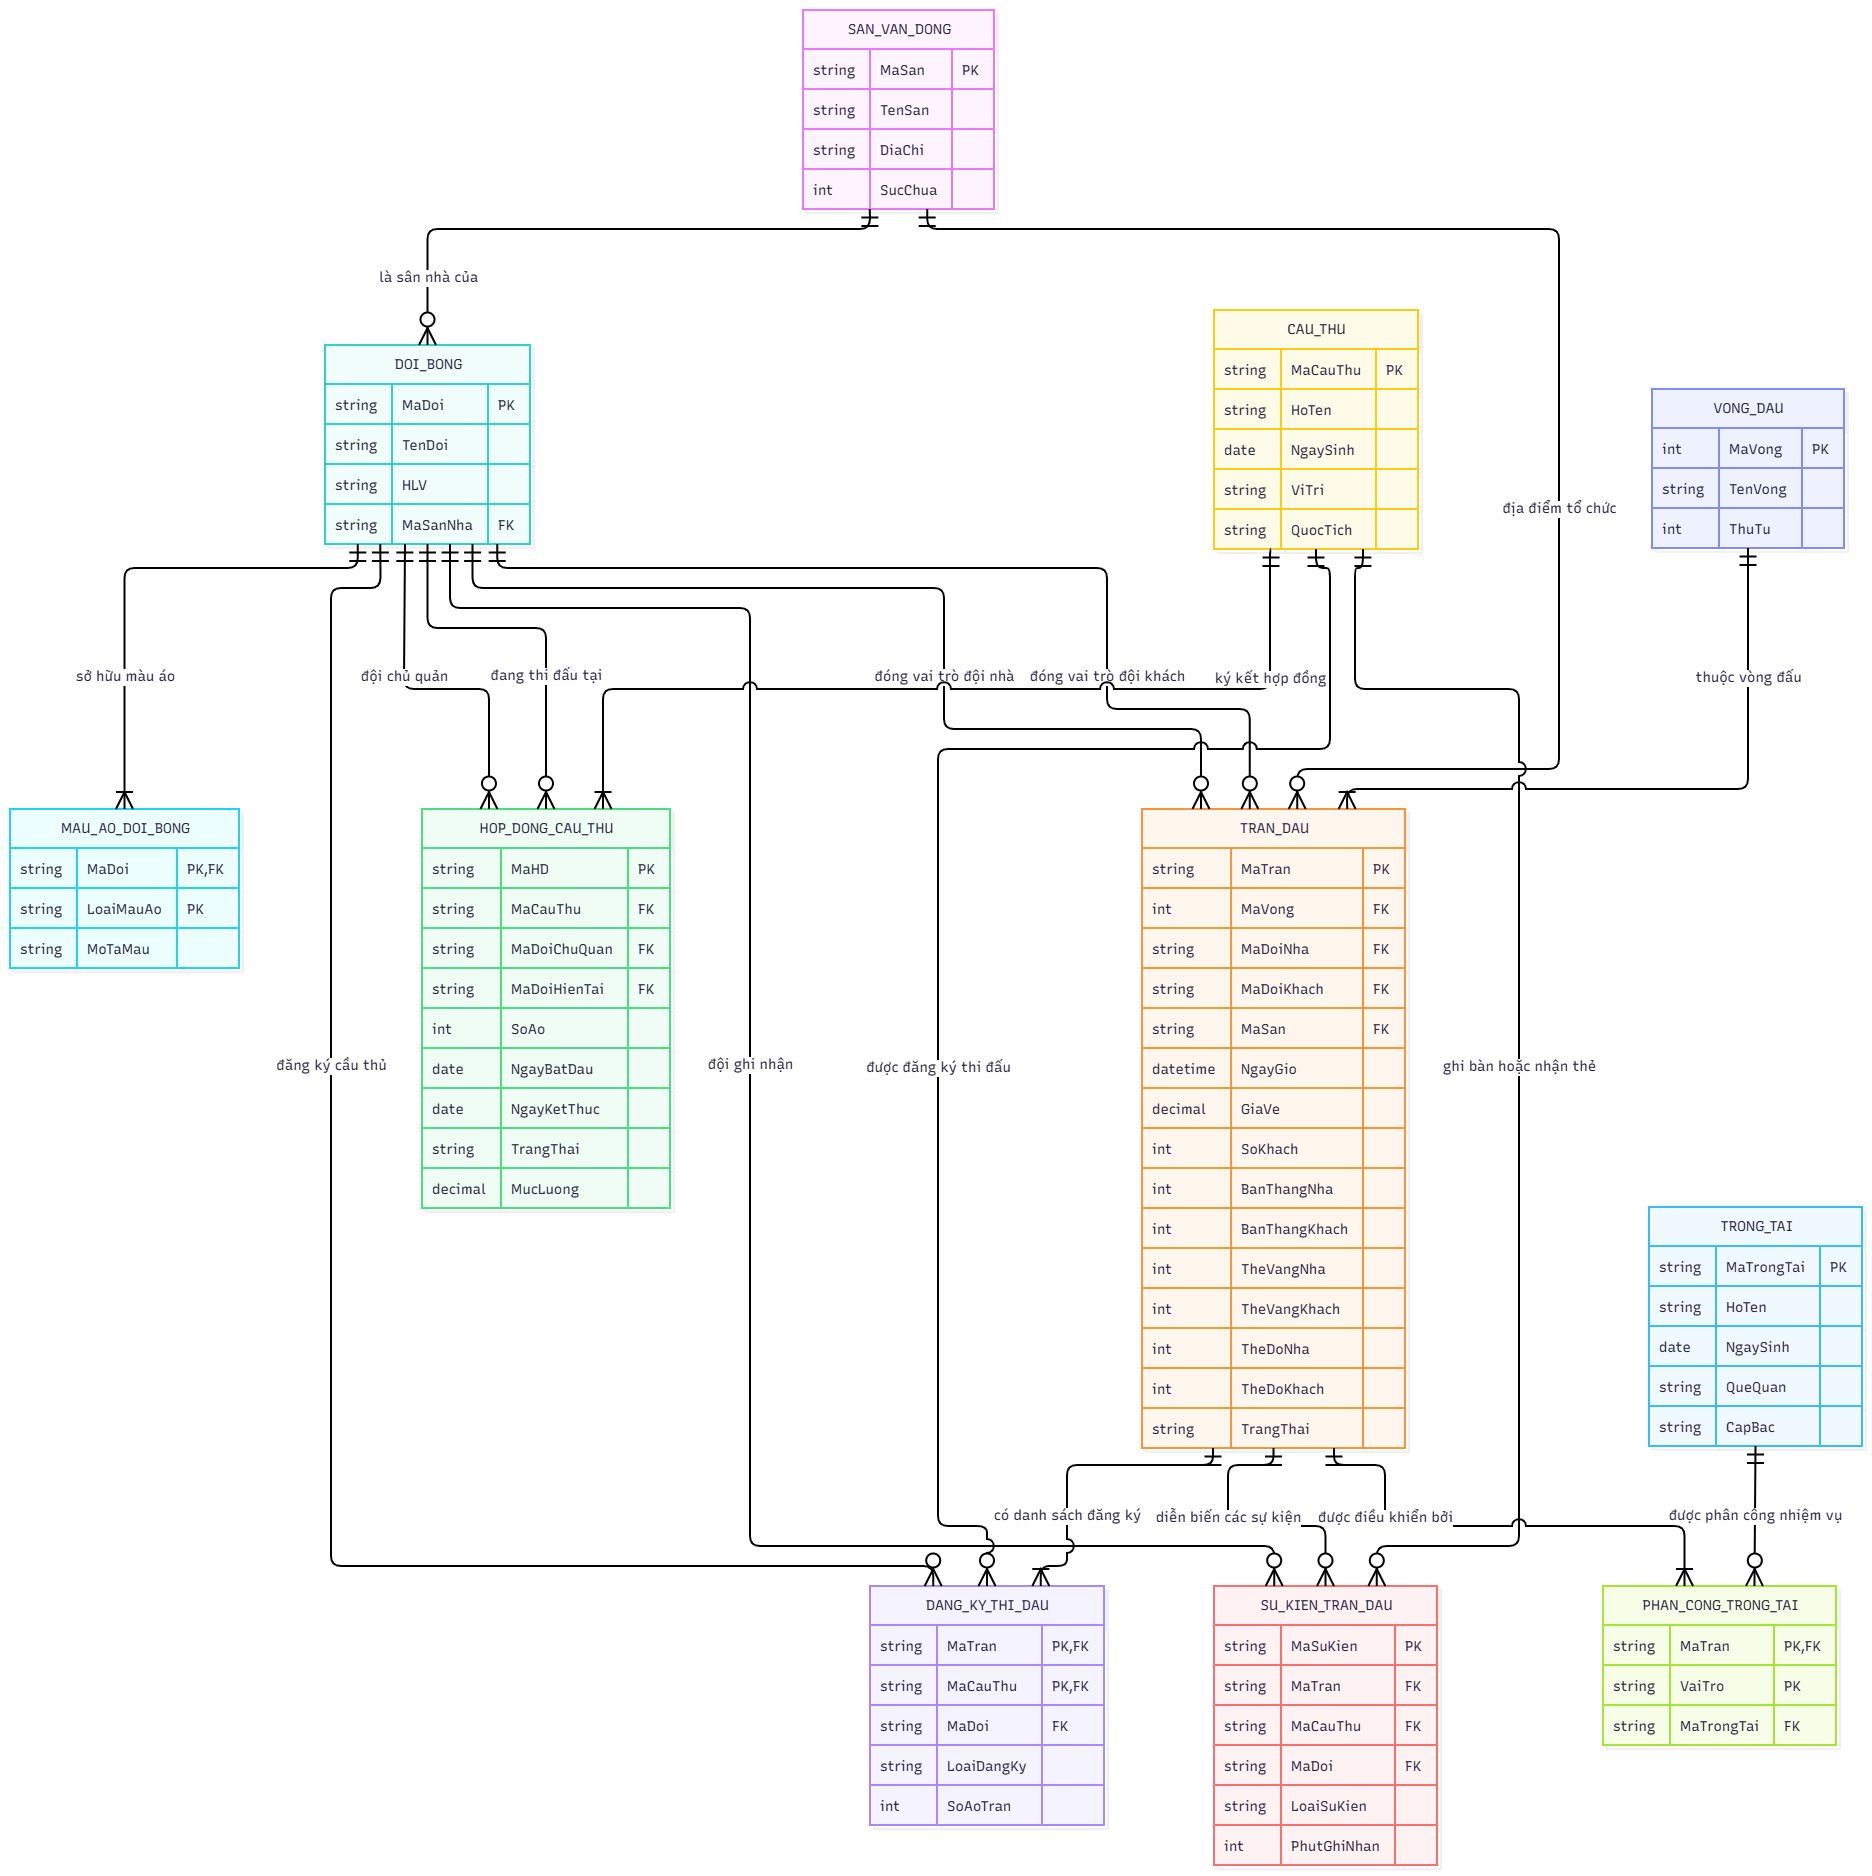
\includegraphics[width=\linewidth]{Figures/ERD.png}
    \caption{Sơ đồ cấu trúc lược đồ quan hệ và mối liên kết khóa}
    \label{fig:er_diagram}
\end{figure}

\chapter{CHUYỂN ĐỔI SANG LƯỢC ĐỒ QUAN HỆ VÀ CHUẨN HÓA BCNF}

\section{Quy tắc ánh xạ từ lược đồ thực thể liên kết sang mô hình quan hệ}

Quá trình chuyển đổi từ lược đồ thực thể liên kết sang các lược đồ quan hệ được thực hiện theo các quy tắc sau:
\begin{enumerate}
    \item \textbf{Ánh xạ tập thực thể mạnh}: Mỗi tập thực thể mạnh gồm \texttt{SAN\_VAN\_DONG}, \texttt{DOI\_BONG}, \texttt{CAU\_THU}, \texttt{TRONG\_TAI}, \texttt{VONG\_DAU} được chuyển thành một quan hệ độc lập. Khóa chính của thực thể trở thành khóa chính của quan hệ tương ứng.
    \item \textbf{Ánh xạ mối kết hợp một -- nhiều}: Được chuyển đổi bằng cách lấy thuộc tính khóa chính của quan hệ phía bên một đưa vào làm thuộc tính khóa ngoại tại quan hệ phía bên nhiều. Ví dụ: Thuộc tính \texttt{MaSanNha} trong quan hệ \texttt{DOI\_BONG} là khóa ngoại tham chiếu đến khóa chính \texttt{MaSan} của quan hệ \texttt{SAN\_VAN\_DONG}.
    \item \textbf{Ánh xạ thuộc tính đa trị và thực thể yếu}: Thuộc tính màu áo của đội bóng được tách thành bảng riêng \texttt{MAU\_AO\_DOI\_BONG}. Khóa chính tổ hợp gồm thuộc tính khóa của đội bóng \texttt{MaDoi} và thuộc tính phân biệt \texttt{LoaiMauAo}.
    \item \textbf{Ánh xạ mối kết hợp nhiều -- nhiều}: Mối kết hợp nhiều -- nhiều giữa \texttt{TRAN\_DAU} và \texttt{TRONG\_TAI} được tách thành quan hệ trung gian \texttt{PHAN\_CONG\_TRONG\_TAI} với khóa chính tổ hợp gồm \texttt{MaTran} và \texttt{VaiTro}. Tương tự, danh sách thi đấu được biểu diễn qua quan hệ \texttt{DANG\_KY\_THI\_DAU}.
\end{enumerate}

\section{Tập hợp các lược đồ quan hệ và liên kết khóa}

Sau khi ánh xạ, hệ thống gồm 11 lược đồ quan hệ. Ký hiệu quy ước: Thuộc tính \underline{\textbf{in đậm gạch chân}} là khóa chính, thuộc tính \textit{in nghiêng} là khóa ngoại.

\begin{enumerate}
    \item $\text{SAN\_VAN\_DONG}(\underline{\mathbf{MaSan}}, \text{TenSan}, \text{DiaChi}, \text{SucChua})$
    
    \item $\text{DOI\_BONG}(\underline{\mathbf{MaDoi}}, \text{TenDoi}, \text{HLV}, \textit{MaSanNha})$\\
    \textit{Khóa ngoại: $\text{MaSanNha} \rightarrow \text{SAN\_VAN\_DONG}(\text{MaSan})$}
    
    \item $\text{MAU\_AO\_DOI\_BONG}(\underline{\mathbf{MaDoi}}, \underline{\mathbf{LoaiMauAo}}, \text{MoTaMau})$\\
    \textit{Khóa ngoại: $\text{MaDoi} \rightarrow \text{DOI\_BONG}(\text{MaDoi})$}
    
    \item $\text{CAU\_THU}(\underline{\mathbf{MaCauThu}}, \text{HoTen}, \text{NgaySinh}, \text{ViTri}, \text{QuocTich})$
    
    \item $\text{HOP\_DONG\_CAU\_THU}(\underline{\mathbf{MaHD}}, \textit{MaCauThu}, \textit{MaDoiChuQuan}, \textit{MaDoiHienTai}, \text{SoAo}, \text{NgayBatDau}, \text{NgayKetThuc}, \text{TrangThai}, \text{MucLuong})$\\
    \textit{Khóa ngoại: $\text{MaCauThu} \rightarrow \text{CAU\_THU}(\text{MaCauThu})$}\\
    \textit{Khóa ngoại: $\text{MaDoiChuQuan} \rightarrow \text{DOI\_BONG}(\text{MaDoi})$}\\
    \textit{Khóa ngoại: $\text{MaDoiHienTai} \rightarrow \text{DOI\_BONG}(\text{MaDoi})$}
    
    \item $\text{TRONG\_TAI}(\underline{\mathbf{MaTrongTai}}, \text{HoTen}, \text{NgaySinh}, \text{QueQuan}, \text{CapBac})$
    
    \item $\text{VONG\_DAU}(\underline{\mathbf{MaVong}}, \text{TenVong}, \text{ThuTu})$
    
    \item $\text{TRAN\_DAU}(\underline{\mathbf{MaTran}}, \textit{MaVong}, \textit{MaDoiNha}, \textit{MaDoiKhach}, \textit{MaSan}, \text{NgayGio}, \text{GiaVe}, \text{SoKhach}, \text{BanThangNha}, \text{BanThangKhach}, \text{TheVangNha}, \text{TheVangKhach}, \text{TheDoNha}, \text{TheDoKhach}, \text{TrangThai})$\\
    \textit{Khóa ngoại: $\text{MaVong} \rightarrow \text{VONG\_DAU}(\text{MaVong})$}\\
    \textit{Khóa ngoại: $\text{MaDoiNha} \rightarrow \text{DOI\_BONG}(\text{MaDoi})$}\\
    \textit{Khóa ngoại: $\text{MaDoiKhach} \rightarrow \text{DOI\_BONG}(\text{MaDoi})$}\\
    \textit{Khóa ngoại: $\text{MaSan} \rightarrow \text{SAN\_VAN\_DONG}(\text{MaSan})$}
    
    \item $\text{PHAN\_CONG\_TRONG\_TAI}(\underline{\mathbf{MaTran}}, \underline{\mathbf{VaiTro}}, \textit{MaTrongTai})$\\
    \textit{Khóa ngoại: $\text{MaTran} \rightarrow \text{TRAN\_DAU}(\text{MaTran})$}\\
    \textit{Khóa ngoại: $\text{MaTrongTai} \rightarrow \text{TRONG\_TAI}(\text{MaTrongTai})$}
    
    \item $\text{DANG\_KY\_THI\_DAU}(\underline{\mathbf{MaTran}}, \underline{\mathbf{MaCauThu}}, \textit{MaDoi}, \text{LoaiDangKy}, \text{SoAoTran})$\\
    \textit{Khóa ngoại: $\text{MaTran} \rightarrow \text{TRAN\_DAU}(\text{MaTran})$}\\
    \textit{Khóa ngoại: $\text{MaCauThu} \rightarrow \text{CAU\_THU}(\text{MaCauThu})$}\\
    \textit{Khóa ngoại: $\text{MaDoi} \rightarrow \text{DOI\_BONG}(\text{MaDoi})$}
    
    \item $\text{SU\_KIEN\_TRAN\_DAU}(\underline{\mathbf{MaSuKien}}, \textit{MaTran}, \textit{MaCauThu}, \textit{MaDoi}, \text{LoaiSuKien}, \text{PhutGhiNhan})$\\
    \textit{Khóa ngoại: $\text{MaTran} \rightarrow \text{TRAN\_DAU}(\text{MaTran})$}\\
    \textit{Khóa ngoại: $\text{MaCauThu} \rightarrow \text{CAU\_THU}(\text{MaCauThu})$}\\
    \textit{Khóa ngoại: $\text{MaDoi} \rightarrow \text{DOI\_BONG}(\text{MaDoi})$}
\end{enumerate}

\begin{figure}[H]
	\centering
	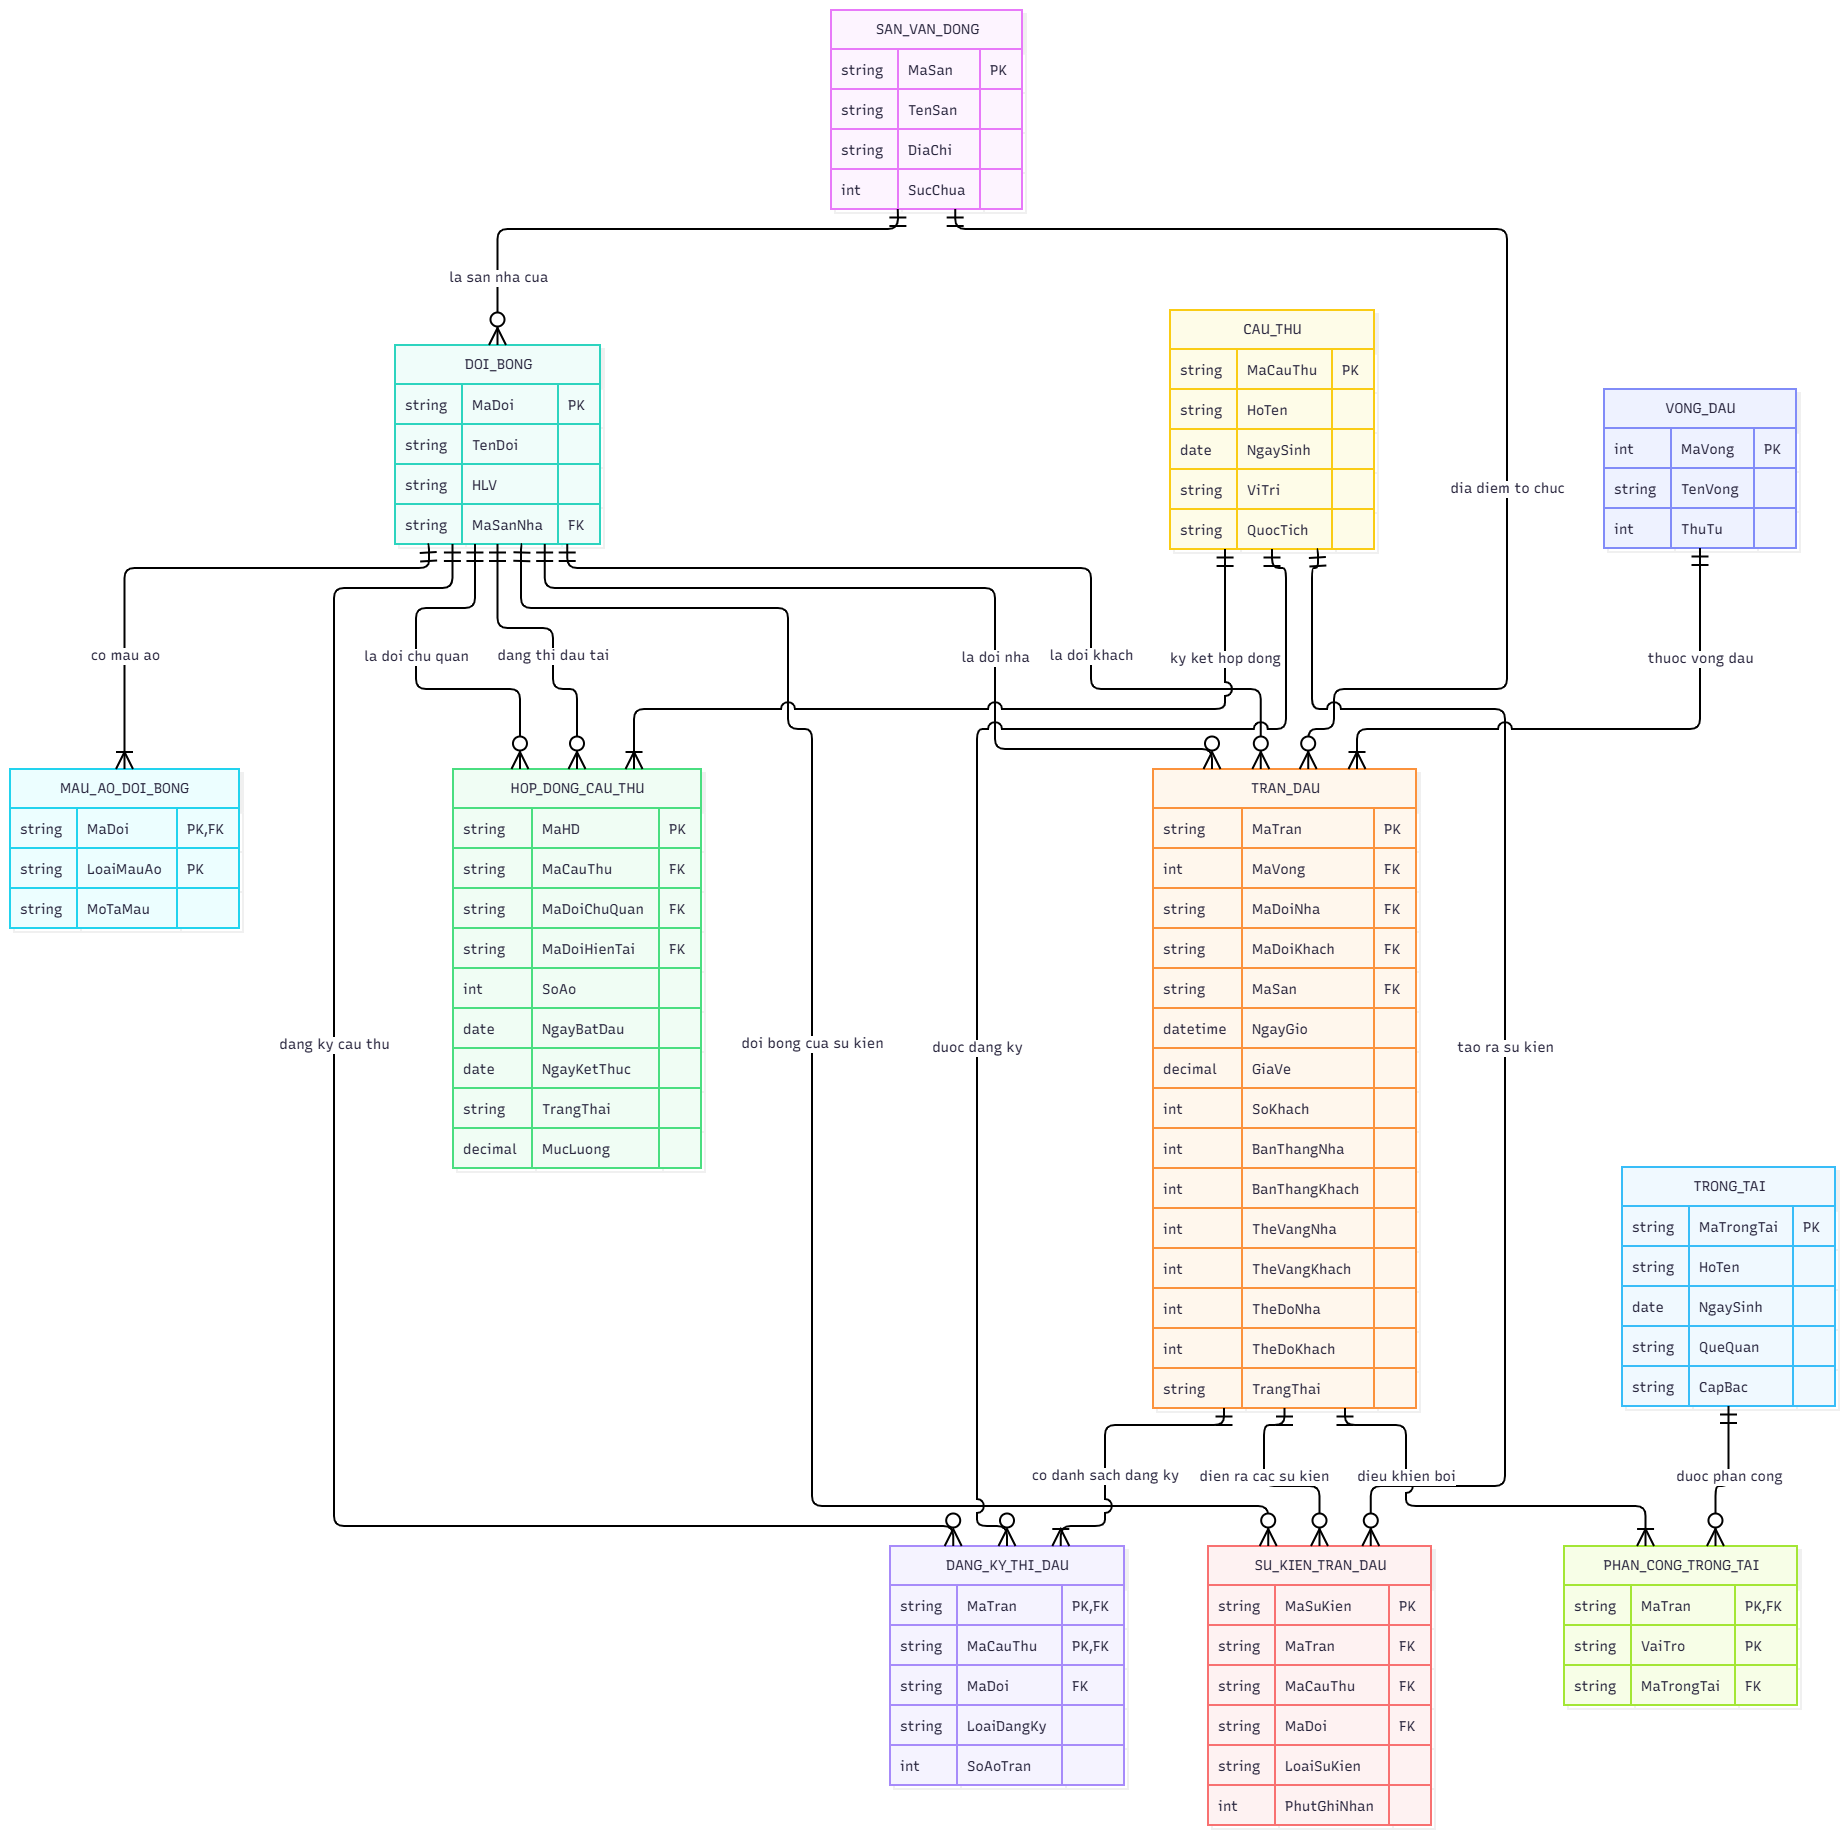
\includegraphics[angle=90, width=0.7\textheight, keepaspectratio]{Figures/RSD.png}
    \caption{Sơ đồ cấu trúc lược đồ quan hệ và mối liên kết khóa}
    \label{fig:relational_diagram}
\end{figure}

\section{Xác định phụ thuộc hàm và chứng minh chuẩn BCNF cho từng lược đồ}

\subsection{Quan hệ SAN\_VAN\_DONG}
\begin{itemize}
    \item Tập thuộc tính: $U = \{\text{MaSan}, \text{TenSan}, \text{DiaChi}, \text{SucChua}\}$.
    \item Tập phụ thuộc hàm tối thiểu $F_1$:
    \begin{align*}
        f_{1.1}: & \quad \text{MaSan} \rightarrow \{\text{TenSan}, \text{DiaChi}, \text{SucChua}\} \\
        f_{1.2}: & \quad \text{TenSan} \rightarrow \{\text{MaSan}, \text{DiaChi}, \text{SucChua}\}
    \end{align*}
    \item Xác định khóa ứng viên:
    $$\text{MaSan}^+ = U \implies \text{MaSan} \text{ là khóa ứng viên.}$$
    $$\text{TenSan}^+ = U \implies \text{TenSan} \text{ là khóa ứng viên.}$$
    \item Kiểm tra điều kiện BCNF:
    \begin{itemize}
        \item Xét $f_{1.1}$: Vế trái $\text{MaSan}$ là siêu khóa.
        \item Xét $f_{1.2}$: Vế trái $\text{TenSan}$ là siêu khóa.
    \end{itemize}
    \item \textbf{Kết luận}: Quan hệ \texttt{SAN\_VAN\_DONG} đạt dạng chuẩn \textbf{BCNF}.
\end{itemize}

\subsection{Quan hệ DOI\_BONG}
\begin{itemize}
    \item Tập thuộc tính: $U = \{\text{MaDoi}, \text{TenDoi}, \text{HLV}, \text{MaSanNha}\}$.
    \item Tập phụ thuộc hàm $F_2$:
    \begin{align*}
        f_{2.1}: & \quad \text{MaDoi} \rightarrow \{\text{TenDoi}, \text{HLV}, \text{MaSanNha}\} \\
        f_{2.2}: & \quad \text{TenDoi} \rightarrow \{\text{MaDoi}, \text{HLV}, \text{MaSanNha}\}
    \end{align*}
    \item Xác định khóa: Khóa ứng viên gồm $\{\text{MaDoi}\}$ và $\{\text{TenDoi}\}$.
    \item Kiểm tra điều kiện BCNF: Cả hai vế trái $\text{MaDoi}$ và $\text{TenDoi}$ đều là siêu khóa của quan hệ.
    \item \textbf{Kết luận}: Quan hệ \texttt{DOI\_BONG} đạt dạng chuẩn \textbf{BCNF}.
\end{itemize}

\subsection{Quan hệ MAU\_AO\_DOI\_BONG}
\begin{itemize}
    \item Tập thuộc tính: $U = \{\text{MaDoi}, \text{LoaiMauAo}, \text{MoTaMau}\}$.
    \item Tập phụ thuộc hàm $F_3$:
    $$f_{3.1}: \quad \{\text{MaDoi}, \text{LoaiMauAo}\} \rightarrow \text{MoTaMau}$$
    \item Khóa ứng viên: $K = \{\text{MaDoi}, \text{LoaiMauAo}\}$ do $\{\text{MaDoi}, \text{LoaiMauAo}\}^+ = U$.
    \item Kiểm tra điều kiện BCNF: Vế trái của phụ thuộc hàm $f_{3.1}$ là khóa chính của quan hệ.
    \item \textbf{Kết luận}: Quan hệ \texttt{MAU\_AO\_DOI\_BONG} đạt dạng chuẩn \textbf{BCNF}.
\end{itemize}

\subsection{Quan hệ CAU\_THU}
\begin{itemize}
    \item Tập thuộc tính: $U = \{\text{MaCauThu}, \text{HoTen}, \text{NgaySinh}, \text{ViTri}, \text{QuocTich}\}$.
    \item Tập phụ thuộc hàm $F_4$:
    $$f_{4.1}: \quad \text{MaCauThu} \rightarrow \{\text{HoTen}, \text{NgaySinh}, \text{ViTri}, \text{QuocTich}\}$$
    \item Khóa ứng viên: $K = \{\text{MaCauThu}\}$.
    \item Kiểm tra điều kiện BCNF: Vế trái $\text{MaCauThu}$ là siêu khóa.
    \item \textbf{Kết luận}: Quan hệ \texttt{CAU\_THU} đạt dạng chuẩn \textbf{BCNF}.
\end{itemize}

\subsection{Quan hệ HOP\_DONG\_CAU\_THU}
\begin{itemize}
    \item Tập thuộc tính: $U = \{\text{MaHD}, \text{MaCauThu}, \text{MaDoiChuQuan}, \text{MaDoiHienTai}, \text{SoAo}, \text{NgayBatDau}, \text{NgayKetThuc}, \text{TrangThai}, \text{MucLuong}\}$.
    \item Tập phụ thuộc hàm $F_5$:
    $$f_{5.1}: \quad \text{MaHD} \rightarrow \{\text{MaCauThu}, \text{MaDoiChuQuan}, \text{MaDoiHienTai}, \text{SoAo}, \text{NgayBatDau}, \text{NgayKetThuc}, \text{TrangThai}, \text{MucLuong}\}$$
    \item Khóa ứng viên: $K = \{\text{MaHD}\}$.
    \item Kiểm tra điều kiện BCNF: Vế trái $\text{MaHD}$ là siêu khóa duy nhất.
    \item \textbf{Kết luận}: Quan hệ \texttt{HOP\_DONG\_CAU\_THU} đạt dạng chuẩn \textbf{BCNF}.
\end{itemize}

\subsection{Quan hệ TRONG\_TAI}
\begin{itemize}
    \item Tập thuộc tính: $U = \{\text{MaTrongTai}, \text{HoTen}, \text{NgaySinh}, \text{QueQuan}, \text{CapBac}\}$.
    \item Tập phụ thuộc hàm $F_6$:
    $$f_{6.1}: \quad \text{MaTrongTai} \rightarrow \{\text{HoTen}, \text{NgaySinh}, \text{QueQuan}, \text{CapBac}\}$$
    \item Khóa ứng viên: $K = \{\text{MaTrongTai}\}$.
    \item Kiểm tra điều kiện BCNF: Vế trái $\text{MaTrongTai}$ là siêu khóa.
    \item \textbf{Kết luận}: Quan hệ \texttt{TRONG\_TAI} đạt dạng chuẩn \textbf{BCNF}.
\end{itemize}

\subsection{Quan hệ VONG\_DAU}
\begin{itemize}
    \item Tập thuộc tính: $U = \{\text{MaVong}, \text{TenVong}, \text{ThuTu}\}$.
    \item Tập phụ thuộc hàm $F_7$:
    \begin{align*}
        f_{7.1}: & \quad \text{MaVong} \rightarrow \{\text{TenVong}, \text{ThuTu}\} \\
        f_{7.2}: & \quad \text{ThuTu} \rightarrow \{\text{MaVong}, \text{TenVong}\}
    \end{align*}
    \item Khóa ứng viên: $K_1 = \{\text{MaVong}\}$, $K_2 = \{\text{ThuTu}\}$.
    \item Kiểm tra điều kiện BCNF: Vế trái của cả hai phụ thuộc hàm đều là siêu khóa.
    \item \textbf{Kết luận}: Quan hệ \texttt{VONG\_DAU} đạt dạng chuẩn \textbf{BCNF}.
\end{itemize}

\subsection{Quan hệ TRAN\_DAU}
\begin{itemize}
    \item Tập thuộc tính:
    $$U = \{\text{MaTran}, \text{MaVong}, \text{MaDoiNha}, \text{MaDoiKhach}, \text{MaSan}, \text{NgayGio}, \text{GiaVe}, \text{SoKhach}, \text{BanThangNha}, \text{BanThangKhach}, \dots\}$$
    \item Tập phụ thuộc hàm $F_8$:
    \begin{align*}
        f_{8.1}: & \quad \text{MaTran} \rightarrow U \setminus \{\text{MaTran}\} \\
        f_{8.2}: & \quad \{\text{MaDoiNha}, \text{MaDoiKhach}\} \rightarrow U \setminus \{\text{MaDoiNha}, \text{MaDoiKhach}\}
    \end{align*}
    (Do mỗi cặp đối đầu sân nhà -- sân khách chỉ diễn ra duy nhất một trận trong cả mùa giải).
    \item Khóa ứng viên: $K_1 = \{\text{MaTran}\}$, $K_2 = \{\text{MaDoiNha}, \text{MaDoiKhach}\}$.
    \item Kiểm tra điều kiện BCNF: Cả hai vế trái $\text{MaTran}$ và $\{\text{MaDoiNha}, \text{MaDoiKhach}\}$ đều là siêu khóa.
    \item \textbf{Kết luận}: Quan hệ \texttt{TRAN\_DAU} đạt dạng chuẩn \textbf{BCNF}.
\end{itemize}

\subsection{Quan hệ PHAN\_CONG\_TRONG\_TAI}
\begin{itemize}
    \item Tập thuộc tính: $U = \{\text{MaTran}, \text{VaiTro}, \text{MaTrongTai}\}$.
    \item Tập phụ thuộc hàm $F_9$:
    \begin{align*}
        f_{9.1}: & \quad \{\text{MaTran}, \text{VaiTro}\} \rightarrow \text{MaTrongTai} \\
        f_{9.2}: & \quad \{\text{MaTran}, \text{MaTrongTai}\} \rightarrow \text{VaiTro}
    \end{align*}
    (Trong một trận đấu, mỗi vai trò chỉ có đúng một trọng tài; và mỗi trọng tài chỉ đảm nhiệm tối đa một vai trò).
    \item Khóa ứng viên: $K_1 = \{\text{MaTran}, \text{VaiTro}\}$, $K_2 = \{\text{MaTran}, \text{MaTrongTai}\}$.
    \item Kiểm tra điều kiện BCNF: Vế trái của $f_{9.1}$ và $f_{9.2}$ đều là siêu khóa của quan hệ.
    \item \textbf{Kết luận}: Quan hệ \texttt{PHAN\_CONG\_TRONG\_TAI} đạt dạng chuẩn \textbf{BCNF}.
\end{itemize}

\subsection{Quan hệ DANG\_KY\_THI\_DAU}
\begin{itemize}
    \item Tập thuộc tính: $U = \{\text{MaTran}, \text{MaCauThu}, \text{MaDoi}, \text{LoaiDangKy}, \text{SoAoTran}\}$.
    \item Tập phụ thuộc hàm $F_{10}$:
    $$f_{10.1}: \quad \{\text{MaTran}, \text{MaCauThu}\} \rightarrow \{\text{MaDoi}, \text{LoaiDangKy}, \text{SoAoTran}\}$$
    \item Khóa ứng viên: $K = \{\text{MaTran}, \text{MaCauThu}\}$.
    \item Kiểm tra điều kiện BCNF: Vế trái $\{\text{MaTran}, \text{MaCauThu}\}$ là siêu khóa duy nhất.
    \item \textbf{Kết luận}: Quan hệ \texttt{DANG\_KY\_THI\_DAU} đạt dạng chuẩn \textbf{BCNF}.
\end{itemize}

\subsection{Quan hệ SU\_KIEN\_TRAN\_DAU}
\begin{itemize}
    \item Tập thuộc tính: $U = \{\text{MaSuKien}, \text{MaTran}, \text{MaCauThu}, \text{MaDoi}, \text{LoaiSuKien}, \text{PhutGhiNhan}\}$.
    \item Tập phụ thuộc hàm $F_{11}$:
    $$f_{11.1}: \quad \text{MaSuKien} \rightarrow \{\text{MaTran}, \text{MaCauThu}, \text{MaDoi}, \text{LoaiSuKien}, \text{PhutGhiNhan}\}$$
    \item Khóa ứng viên: $K = \{\text{MaSuKien}\}$.
    \item Kiểm tra điều kiện BCNF: Vế trái $\text{MaSuKien}$ là siêu khóa.
    \item \textbf{Kết luận}: Quan hệ \texttt{SU\_KIEN\_TRAN\_DAU} đạt dạng chuẩn \textbf{BCNF}.
\end{itemize}

% \section{Phân tích thuật toán tách chuẩn BCNF}

% Mục này trình bày một ví dụ thiết kế chưa chuẩn hóa và các bước áp dụng thuật toán tách để đưa quan hệ về dạng chuẩn BCNF.

% \subsection{Tình huống thiết kế vi phạm chuẩn hóa}
% Giả sử người thiết kế gộp chung thông tin của Trận đấu và Sân vận động vào trong một bảng duy nhất:
% $$R_{\text{Gop}}(\underline{\text{MaTran}}, \text{NgayGio}, \text{MaSan}, \text{TenSan}, \text{DiaChi}, \text{SucChua})$$

% Tập phụ thuộc hàm trên $R_{\text{Gop}}$ gồm:
% \begin{align*}
%     f_1: & \quad \text{MaTran} \rightarrow \{\text{NgayGio}, \text{MaSan}, \text{TenSan}, \text{DiaChi}, \text{SucChua}\} \\
%     f_2: & \quad \text{MaSan} \rightarrow \{\text{TenSan}, \text{DiaChi}, \text{SucChua}\}
% \end{align*}

% \paragraph{Phân tích vi phạm BCNF:}
% \begin{itemize}
%     \item Khóa chính duy nhất của $R_{\text{Gop}}$ là $\{\text{MaTran}\}$.
%     \item Xét phụ thuộc hàm $f_2: \text{MaSan} \rightarrow \{\text{TenSan}, \text{DiaChi}, \text{SucChua}\}$. Vế trái $\text{MaSan}$ không phải là siêu khóa của $R_{\text{Gop}}$ (vì bao đóng của $\text{MaSan}$ không chứa thuộc tính $\text{MaTran}$ và $\text{NgayGio}$).
%     \item Do đó, quan hệ $R_{\text{Gop}}$ vi phạm định nghĩa dạng chuẩn BCNF và vi phạm dạng chuẩn 3 do tồn tại phụ thuộc bắc cầu.
%     \item Hậu quả là thông tin tên sân, địa chỉ, sức chứa bị lặp lại ở mọi trận đấu diễn ra trên sân đó, dẫn đến các dị thường khi thêm, sửa hoặc xóa dữ liệu.
% \end{itemize}

% \subsection{Các bước thực hiện thuật toán tách BCNF}
% Thuật toán tách được thực hiện như sau:
% \begin{itemize}
%     \item \textbf{Bước 1}: Chọn phụ thuộc hàm vi phạm điều kiện BCNF là $f_2: \text{MaSan} \rightarrow \{\text{TenSan}, \text{DiaChi}, \text{SucChua}\}$.
%     \item \textbf{Bước 2}: Tách $R_{\text{Gop}}$ thành hai lược đồ quan hệ con $R_1$ và $R_2$:
%     $$R_1 = \{\underline{\mathbf{MaSan}}, \text{TenSan}, \text{DiaChi}, \text{SucChua}\} \equiv \text{SAN\_VAN\_DONG}$$
%     $$R_2 = \{\underline{\mathbf{MaTran}}, \text{NgayGio}, \textit{MaSan}\} \equiv \text{TRAN\_DAU\_RUT\_GON}$$
%     \item \textbf{Bước 3}: Kiểm tra các tính chất của phép tách:
%     \begin{enumerate}
%         \item \textit{Tính kết nối không mất mát thông tin}:
%         Giao của hai quan hệ là $R_1 \cap R_2 = \{\text{MaSan}\}$. Vì $\text{MaSan}$ là khóa chính của $R_1$ nên phép tách bảo toàn toàn bộ dữ liệu ban đầu:
%         $$R_{\text{Gop}} = R_1 \bowtie R_2.$$
%         \item \textit{Tính bảo toàn phụ thuộc hàm}: Các phụ thuộc hàm trong tập ban đầu đều được duy trì trong các bảng con.
%         \item \textit{Kiểm tra lại điều kiện BCNF}: Cả hai quan hệ $R_1$ và $R_2$ đều thỏa mãn dạng chuẩn BCNF.
%     \end{enumerate}
% \end{itemize}

% Kết quả này cho thấy việc tách các thực thể theo mô hình thiết kế đã loại bỏ hoàn toàn dư thừa dữ liệu.

\chapter{CÀI ĐẶT CƠ SỞ DỮ LIỆU, BỘ KÍCH HOẠT VÀ THỦ TỤC GIAO DỊCH}

\section{Môi trường cài đặt và cấu trúc bảng dữ liệu}

Hệ thống cơ sở dữ liệu được cài đặt trên hệ quản trị PostgreSQL. Toàn bộ 11 bảng dữ liệu được tạo lập với đầy đủ các thuộc tính, kiểu dữ liệu, các ràng buộc khóa chính, khóa ngoại và ràng buộc kiểm tra miền giá trị.

\begin{lstlisting}[language=SQL, caption={Kịch bản tạo bảng và ràng buộc toàn vẹn}]
-- Bang san van dong
CREATE TABLE SAN_VAN_DONG (
    MaSan VARCHAR(10) PRIMARY KEY,
    TenSan VARCHAR(100) NOT NULL UNIQUE,
    DiaChi VARCHAR(200) NOT NULL,
    SucChua INT NOT NULL CHECK (SucChua > 0)
);

-- Bang doi bong
CREATE TABLE DOI_BONG (
    MaDoi VARCHAR(10) PRIMARY KEY,
    TenDoi VARCHAR(100) NOT NULL UNIQUE,
    HLV VARCHAR(100) NOT NULL,
    MaSanNha VARCHAR(10) NOT NULL REFERENCES SAN_VAN_DONG(MaSan)
);

-- Bang mau ao doi bong
CREATE TABLE MAU_AO_DOI_BONG (
    MaDoi VARCHAR(10) NOT NULL REFERENCES DOI_BONG(MaDoi) ON DELETE CASCADE,
    LoaiMauAo VARCHAR(20) NOT NULL CHECK (LoaiMauAo IN ('SanNha', 'SanKhach', 'Phu')),
    MoTaMau VARCHAR(50) NOT NULL,
    PRIMARY KEY (MaDoi, LoaiMauAo)
);

-- Bang hop dong cau thu voi rang buoc so ao tu 1 den 35
CREATE TABLE HOP_DONG_CAU_THU (
    MaHD VARCHAR(10) PRIMARY KEY,
    MaCauThu VARCHAR(10) NOT NULL REFERENCES CAU_THU(MaCauThu),
    MaDoiChuQuan VARCHAR(10) NOT NULL REFERENCES DOI_BONG(MaDoi),
    MaDoiHienTai VARCHAR(10) NOT NULL REFERENCES DOI_BONG(MaDoi),
    SoAo INT NOT NULL CHECK (SoAo BETWEEN 1 AND 35),
    NgayBatDau DATE NOT NULL,
    NgayKetThuc DATE NOT NULL,
    TrangThai VARCHAR(20) NOT NULL CHECK (TrangThai IN ('ChinhThuc', 'ChoMuon')),
    MucLuong DECIMAL(15, 2) DEFAULT 0 CHECK (MucLuong >= 0),
    CHECK (NgayKetThuc > NgayBatDau)
);
\end{lstlisting}

\section{Cài đặt năm bộ kích hoạt kiểm tra toàn vẹn nghiệp vụ}

Để đảm bảo các quy tắc nghiệp vụ phức tạp của bài toán luôn được thỏa mãn trong mọi thao tác cập nhật dữ liệu, hệ thống cài đặt năm bộ kích hoạt sau:

\subsection{Bộ kích hoạt kiểm tra số áo duy nhất trong cùng đội bóng}
Mỗi cầu thủ trong cùng một đội bóng phải có số áo khác nhau trong thời gian hợp đồng có hiệu lực. Bộ kích hoạt tự động chặn việc đăng ký trùng số áo:

\begin{lstlisting}[language=SQL, caption={Bộ kích hoạt kiểm tra số áo duy nhất trong đội}]
CREATE OR REPLACE FUNCTION fn_check_so_ao_duy_nhat()
RETURNS TRIGGER AS $$
DECLARE
    v_trung_so_ao INT;
BEGIN
    SELECT COUNT(*) INTO v_trung_so_ao
    FROM HOP_DONG_CAU_THU
    WHERE MaDoiHienTai = NEW.MaDoiHienTai
      AND SoAo = NEW.SoAo
      AND MaCauThu <> NEW.MaCauThu
      AND NOT (NgayKetThuc < NEW.NgayBatDau OR NgayBatDau > NEW.NgayKetThuc);

    IF v_trung_so_ao > 0 THEN
        RAISE EXCEPTION 'Loi nghiep vu: So ao da duoc dang ky cho cau thu khac!';
    END IF;
    RETURN NEW;
END;
$$ LANGUAGE plpgsql;

CREATE TRIGGER trg_check_so_ao_duy_nhat
BEFORE INSERT OR UPDATE OF SoAo, MaDoiHienTai, NgayBatDau, NgayKetThuc
ON HOP_DONG_CAU_THU
FOR EACH ROW EXECUTE FUNCTION fn_check_so_ao_duy_nhat();
\end{lstlisting}

\subsection{Bộ kích hoạt kiểm tra giới hạn tối đa 30 cầu thủ mỗi đội}
Một đội bóng chỉ được đăng ký tối đa 30 cầu thủ thi đấu trong một mùa giải. Bộ kích hoạt tự động đếm số lượng cầu thủ hiện tại trước khi thêm mới hoặc chuyển nhượng:

\begin{lstlisting}[language=SQL, caption={Bộ kích hoạt giới hạn tối đa 30 cầu thủ}]
CREATE OR REPLACE FUNCTION fn_check_gioi_han_30_cau_thu()
RETURNS TRIGGER AS $$
DECLARE
    v_so_luong INT;
BEGIN
    SELECT COUNT(*) INTO v_so_luong
    FROM HOP_DONG_CAU_THU
    WHERE MaDoiHienTai = NEW.MaDoiHienTai
      AND MaCauThu <> NEW.MaCauThu
      AND CURRENT_DATE BETWEEN NgayBatDau AND NgayKetThuc;

    IF v_so_luong >= 30 THEN
        RAISE EXCEPTION 'Loi nghiep vu: Doi bong da dat toi da 30 cau thu!';
    END IF;
    RETURN NEW;
END;
$$ LANGUAGE plpgsql;

CREATE TRIGGER trg_check_gioi_han_30_cau_thu
BEFORE INSERT OR UPDATE OF MaDoiHienTai
ON HOP_DONG_CAU_THU
FOR EACH ROW EXECUTE FUNCTION fn_check_gioi_han_30_cau_thu();
\end{lstlisting}

\subsection{Bộ kích hoạt giới hạn một trọng tài điều khiển tối đa một trận mỗi vòng}
Trong cùng một vòng đấu, một trọng tài chỉ được phép điều khiển tối đa một trận đấu nhằm bảo đảm tính công bằng và thể lực:

\begin{lstlisting}[language=SQL, caption={Bộ kích hoạt giới hạn nhiệm vụ trọng tài theo vòng}]
CREATE OR REPLACE FUNCTION fn_check_trong_tai_toi_da_1_tran_1_vong()
RETURNS TRIGGER AS $$
DECLARE
    v_ma_vong INT;
    v_so_tran INT;
BEGIN
    SELECT MaVong INTO v_ma_vong
    FROM TRAN_DAU
    WHERE MaTran = NEW.MaTran;

    SELECT COUNT(*) INTO v_so_tran
    FROM PHAN_CONG_TRONG_TAI pc
    JOIN TRAN_DAU td ON pc.MaTran = td.MaTran
    WHERE pc.MaTrongTai = NEW.MaTrongTai
      AND td.MaVong = v_ma_vong
      AND td.MaTran <> NEW.MaTran;

    IF v_so_tran > 0 THEN
        RAISE EXCEPTION 'Loi nghiep vu: Trong tai da dieu khien tran khac trong cung vong!';
    END IF;
    RETURN NEW;
END;
$$ LANGUAGE plpgsql;

CREATE TRIGGER trg_check_trong_tai_toi_da_1_tran_1_vong
BEFORE INSERT OR UPDATE OF MaTrongTai, MaTran
ON PHAN_CONG_TRONG_TAI
FOR EACH ROW EXECUTE FUNCTION fn_check_trong_tai_toi_da_1_tran_1_vong();
\end{lstlisting}

\subsection{Bộ kích hoạt giới hạn tối đa 18 cầu thủ đăng ký mỗi trận}
Mỗi đội bóng tham gia trận đấu chỉ được đăng ký tối đa 18 cầu thủ gồm đội hình đá chính và danh sách dự bị:

\begin{lstlisting}[language=SQL, caption={Bộ kích hoạt giới hạn 18 cầu thủ đăng ký trận đấu}]
CREATE OR REPLACE FUNCTION fn_check_dang_ky_toi_da_18_cau_thu()
RETURNS TRIGGER AS $$
DECLARE
    v_so_cau_thu INT;
BEGIN
    SELECT COUNT(*) INTO v_so_cau_thu
    FROM DANG_KY_THI_DAU
    WHERE MaTran = NEW.MaTran
      AND MaDoi = NEW.MaDoi
      AND MaCauThu <> NEW.MaCauThu;

    IF v_so_cau_thu >= 18 THEN
        RAISE EXCEPTION 'Loi nghiep vu: Doi bong da dang ky du toi da 18 cau thu!';
    END IF;
    RETURN NEW;
END;
$$ LANGUAGE plpgsql;

CREATE TRIGGER trg_check_dang_ky_toi_da_18_cau_thu
BEFORE INSERT ON DANG_KY_THI_DAU
FOR EACH ROW EXECUTE FUNCTION fn_check_dang_ky_toi_da_18_cau_thu();
\end{lstlisting}

\subsection{Bộ kích hoạt kiểm tra tính khớp giữa sự kiện và kết quả trận đấu}
Khi kết thúc trận đấu, tổng số bàn thắng, thẻ vàng và thẻ đỏ được ghi nhận trong bảng sự kiện chi tiết bắt buộc phải khớp chính xác với tỉ số và số thẻ ghi nhận trong bảng trận đấu:

\begin{lstlisting}[language=SQL, caption={Bộ kích hoạt kiểm tra tính khớp giữa kết quả và sự kiện}]
CREATE OR REPLACE FUNCTION fn_check_khop_ban_thang_va_the()
RETURNS TRIGGER AS $$
DECLARE
    v_ban_nha INT;
    v_ban_khach INT;
    v_the_vang_nha INT;
    v_the_vang_khach INT;
    v_the_do_nha INT;
    v_the_do_khach INT;
BEGIN
    IF NEW.TrangThai = 'DaKetThuc' THEN
        SELECT COUNT(*) INTO v_ban_nha FROM SU_KIEN_TRAN_DAU
        WHERE MaTran = NEW.MaTran AND MaDoi = NEW.MaDoiNha AND LoaiSuKien = 'BanThang';

        SELECT COUNT(*) INTO v_ban_khach FROM SU_KIEN_TRAN_DAU
        WHERE MaTran = NEW.MaTran AND MaDoi = NEW.MaDoiKhach AND LoaiSuKien = 'BanThang';

        SELECT COUNT(*) INTO v_the_vang_nha FROM SU_KIEN_TRAN_DAU
        WHERE MaTran = NEW.MaTran AND MaDoi = NEW.MaDoiNha AND LoaiSuKien = 'TheVang';

        SELECT COUNT(*) INTO v_the_vang_khach FROM SU_KIEN_TRAN_DAU
        WHERE MaTran = NEW.MaTran AND MaDoi = NEW.MaDoiKhach AND LoaiSuKien = 'TheVang';

        SELECT COUNT(*) INTO v_the_do_nha FROM SU_KIEN_TRAN_DAU
        WHERE MaTran = NEW.MaTran AND MaDoi = NEW.MaDoiNha AND LoaiSuKien = 'TheDo';

        SELECT COUNT(*) INTO v_the_do_khach FROM SU_KIEN_TRAN_DAU
        WHERE MaTran = NEW.MaTran AND MaDoi = NEW.MaDoiKhach AND LoaiSuKien = 'TheDo';

        IF v_ban_nha <> NEW.BanThangNha OR v_ban_khach <> NEW.BanThangKhach THEN
            RAISE EXCEPTION 'Loi toan ven: So ban thang trong su kien khong khop voi ti so tran dau!';
        END IF;

        IF v_the_vang_nha <> NEW.TheVangNha OR v_the_vang_khach <> NEW.TheVangKhach OR
           v_the_do_nha <> NEW.TheDoNha OR v_the_do_khach <> NEW.TheDoKhach THEN
            RAISE EXCEPTION 'Loi toan ven: So the phat trong su kien khong khop voi tong so the tran dau!';
        END IF;
    END IF;
    RETURN NEW;
END;
$$ LANGUAGE plpgsql;

CREATE TRIGGER trg_check_khop_ban_thang_va_the
AFTER INSERT OR UPDATE OF TrangThai, BanThangNha, BanThangKhach
ON TRAN_DAU
FOR EACH ROW EXECUTE FUNCTION fn_check_khop_ban_thang_va_the();
\end{lstlisting}

\section{Cài đặt năm thủ tục giao dịch thực thi nghiệp vụ}

Các quy trình nghiệp vụ trọng yếu được cài đặt dưới dạng các thủ tục giao dịch nhằm bảo đảm tính nguyên tử và nhất quán của dữ liệu:

\subsection{Thủ tục giao dịch tạo lịch thi đấu}
Khởi tạo lịch thi đấu cho một trận đấu, kiểm tra điều kiện hai đội không trùng nhau, cặp đấu chưa từng diễn ra trên sân nhà này trong mùa giải, và sân vận động không bị trùng giờ:

\begin{lstlisting}[language=SQL, caption={Thủ tục giao dịch lập lịch thi đấu}]
CREATE OR REPLACE PROCEDURE sp_tao_lich_thi_dau(
    p_ma_tran VARCHAR(10),
    p_ma_vong INT,
    p_ma_doi_nha VARCHAR(10),
    p_ma_doi_khach VARCHAR(10),
    p_ma_san VARCHAR(10),
    p_ngay_gio TIMESTAMP,
    p_gia_ve DECIMAL(12, 2)
)
LANGUAGE plpgsql AS $$
DECLARE
    v_da_ton_tai INT;
    v_trung_lich_san INT;
BEGIN
    IF p_ma_doi_nha = p_ma_doi_khach THEN
        RAISE EXCEPTION 'Loi: Doi chu nha va doi khach khong duoc trung nhau!';
    END IF;

    SELECT COUNT(*) INTO v_da_ton_tai FROM TRAN_DAU
    WHERE MaDoiNha = p_ma_doi_nha AND MaDoiKhach = p_ma_doi_khach;

    IF v_da_ton_tai > 0 THEN
        RAISE EXCEPTION 'Loi: Cap dau nay da duoc xep lich truoc do!';
    END IF;

    SELECT COUNT(*) INTO v_trung_lich_san FROM TRAN_DAU
    WHERE MaSan = p_ma_san AND ABS(EXTRACT(EPOCH FROM (NgayGio - p_ngay_gio))) < 14400;

    IF v_trung_lich_san > 0 THEN
        RAISE EXCEPTION 'Loi: San van dong da co tran dau trong khoang gio nay!';
    END IF;

    INSERT INTO TRAN_DAU (
        MaTran, MaVong, MaDoiNha, MaDoiKhach, MaSan, NgayGio, GiaVe, TrangThai
    ) VALUES (
        p_ma_tran, p_ma_vong, p_ma_doi_nha, p_ma_doi_khach, p_ma_san, p_ngay_gio, p_gia_ve, 'ChuaDienRa'
    );
END;
$$;
\end{lstlisting}

\subsection{Thủ tục giao dịch phân công tổ bốn trọng tài}
Phân công đồng thời cả bốn trọng tài cho một trận đấu trong một giao dịch duy nhất, bảo đảm bốn trọng tài là các cá nhân phân biệt:

\begin{lstlisting}[language=SQL, caption={Thủ tục giao dịch phân công tổ trọng tài}]
CREATE OR REPLACE PROCEDURE sp_phan_cong_to_trong_tai(
    p_ma_tran VARCHAR(10),
    p_tt_chinh VARCHAR(10),
    p_tt_bien1 VARCHAR(10),
    p_tt_bien2 VARCHAR(10),
    p_tt_ban VARCHAR(10)
)
LANGUAGE plpgsql AS $$
BEGIN
    IF p_tt_chinh IN (p_tt_bien1, p_tt_bien2, p_tt_ban) OR
       p_tt_bien1 IN (p_tt_bien2, p_tt_ban) OR
       p_tt_bien2 = p_tt_ban THEN
        RAISE EXCEPTION 'Loi: Bon trong tai phai la cac ca nhan phan biet!';
    END IF;

    DELETE FROM PHAN_CONG_TRONG_TAI WHERE MaTran = p_ma_tran;

    INSERT INTO PHAN_CONG_TRONG_TAI (MaTran, VaiTro, MaTrongTai) VALUES
    (p_ma_tran, 'Chinh', p_tt_chinh),
    (p_ma_tran, 'Bien1', p_tt_bien1),
    (p_ma_tran, 'Bien2', p_tt_bien2),
    (p_ma_tran, 'Ban', p_tt_ban);
END;
$$;
\end{lstlisting}

\subsection{Thủ tục giao dịch đăng ký cầu thủ thi đấu}
Đăng ký danh sách thi đấu cho trận, kiểm tra cầu thủ có hợp đồng hợp lệ tại đội bóng và tự động trích xuất số áo:

\begin{lstlisting}[language=SQL, caption={Thủ tục giao dịch đăng ký cầu thủ trận đấu}]
CREATE OR REPLACE PROCEDURE sp_dang_ky_cau_thu_tran(
    p_ma_tran VARCHAR(10),
    p_ma_doi VARCHAR(10),
    p_ma_cau_thu VARCHAR(10),
    p_loai_dang_ky VARCHAR(20)
)
LANGUAGE plpgsql AS $$
DECLARE
    v_so_ao INT;
BEGIN
    SELECT SoAo INTO v_so_ao
    FROM HOP_DONG_CAU_THU
    WHERE MaCauThu = p_ma_cau_thu
      AND MaDoiHienTai = p_ma_doi
      AND CURRENT_DATE BETWEEN NgayBatDau AND NgayKetThuc;

    IF v_so_ao IS NULL THEN
        RAISE EXCEPTION 'Loi: Cau thu khong thuoc bien che hop le cua doi bong!';
    END IF;

    INSERT INTO DANG_KY_THI_DAU (MaTran, MaCauThu, MaDoi, LoaiDangKy, SoAoTran)
    VALUES (p_ma_tran, p_ma_cau_thu, p_ma_doi, p_loai_dang_ky, v_so_ao);
END;
$$;
\end{lstlisting}

\subsection{Thủ tục giao dịch ghi nhận kết quả trận đấu}
Cập nhật kết quả chung cuộc, số khán giả theo dõi và chuyển trạng thái sang đã kết thúc:

\begin{lstlisting}[language=SQL, caption={Thủ tục giao dịch hoàn tất trận đấu}]
CREATE OR REPLACE PROCEDURE sp_ghi_nhan_ket_qua_tran_dau(
    p_ma_tran VARCHAR(10),
    p_so_khach INT,
    p_ban_nha INT,
    p_ban_khach INT,
    p_the_vang_nha INT,
    p_the_vang_khach INT,
    p_the_do_nha INT,
    p_the_do_khach INT
)
LANGUAGE plpgsql AS $$
DECLARE
    v_ngay_gio TIMESTAMP;
BEGIN
    SELECT NgayGio INTO v_ngay_gio FROM TRAN_DAU WHERE MaTran = p_ma_tran;

    IF v_ngay_gio > CURRENT_TIMESTAMP THEN
        RAISE EXCEPTION 'Loi: Khong the ket thuc tran dau o thoi diem tuong lai!';
    END IF;

    UPDATE TRAN_DAU
    SET SoKhach = p_so_khach,
        BanThangNha = p_ban_nha,
        BanThangKhach = p_ban_khach,
        TheVangNha = p_the_vang_nha,
        TheVangKhach = p_the_vang_khach,
        TheDoNha = p_the_do_nha,
        TheDoKhach = p_the_do_khach,
        TrangThai = 'DaKetThuc'
    WHERE MaTran = p_ma_tran;
END;
$$;
\end{lstlisting}

\subsection{Thủ tục giao dịch chuyển nhượng hoặc cho mượn cầu thủ}
Cập nhật thời hạn kết thúc của hợp đồng cũ và khởi tạo hợp đồng thi đấu mới tại đội bóng tiếp nhận:

\begin{lstlisting}[language=SQL, caption={Thủ tục giao dịch chuyển nhượng hoặc cho mượn cầu thủ}]
CREATE OR REPLACE PROCEDURE sp_chuyen_nhuong_cho_muon_cau_thu(
    p_ma_hd_moi VARCHAR(10),
    p_ma_cau_thu VARCHAR(10),
    p_ma_doi_chu_quan VARCHAR(10),
    p_ma_doi_moi VARCHAR(10),
    p_so_ao_moi INT,
    p_ngay_bat_dau DATE,
    p_ngay_ket_thuc DATE,
    p_trang_thai VARCHAR(20),
    p_muc_luong DECIMAL(15, 2)
)
LANGUAGE plpgsql AS $$
BEGIN
    UPDATE HOP_DONG_CAU_THU
    SET NgayKetThuc = p_ngay_bat_dau - INTERVAL '1 day'
    WHERE MaCauThu = p_ma_cau_thu AND NgayKetThuc >= p_ngay_bat_dau;

    INSERT INTO HOP_DONG_CAU_THU (
        MaHD, MaCauThu, MaDoiChuQuan, MaDoiHienTai, 
        SoAo, NgayBatDau, NgayKetThuc, TrangThai, MucLuong
    ) VALUES (
        p_ma_hd_moi, p_ma_cau_thu, p_ma_doi_chu_quan, p_ma_doi_moi,
        p_so_ao_moi, p_ngay_bat_dau, p_ngay_ket_thuc, p_trang_thai, p_muc_luong
    );
END;
$$;
\end{lstlisting}

\section{Cài đặt các khung nhìn và hàm nghiệp vụ thống kê}

\subsection{Khung nhìn bảng xếp hạng mùa giải}
Bảng xếp hạng được tính toán tự động từ tất cả các trận đấu đã kết thúc, áp dụng thể thức thắng 3 điểm, hòa 1 điểm, thua 0 điểm và sắp xếp theo đúng các tiêu chí ưu tiên:

\begin{lstlisting}[language=SQL, caption={Khung nhìn bảng xếp hạng mùa giải}]
CREATE OR REPLACE VIEW vw_bang_xep_hang AS
WITH TranDauKetThuc AS (
    SELECT MaDoiNha AS MaDoi, 1 AS SoTran,
        CASE WHEN BanThangNha > BanThangKhach THEN 1 ELSE 0 END AS Thang,
        CASE WHEN BanThangNha = BanThangKhach THEN 1 ELSE 0 END AS Hoa,
        CASE WHEN BanThangNha < BanThangKhach THEN 1 ELSE 0 END AS Thua,
        BanThangNha AS BanThang, BanThangKhach AS BanThua,
        0 AS ThangSanKhach, TheDoNha AS TheDo, TheVangNha AS TheVang
    FROM TRAN_DAU WHERE TrangThai = 'DaKetThuc'
    UNION ALL
    SELECT MaDoiKhach AS MaDoi, 1 AS SoTran,
        CASE WHEN BanThangKhach > BanThangNha THEN 1 ELSE 0 END AS Thang,
        CASE WHEN BanThangKhach = BanThangNha THEN 1 ELSE 0 END AS Hoa,
        CASE WHEN BanThangKhach < BanThangNha THEN 1 ELSE 0 END AS Thua,
        BanThangKhach AS BanThang, BanThangNha AS BanThua,
        CASE WHEN BanThangKhach > BanThangNha THEN 1 ELSE 0 END AS ThangSanKhach,
        TheDoKhach AS TheDo, TheVangKhach AS TheVang
    FROM TRAN_DAU WHERE TrangThai = 'DaKetThuc'
)
SELECT 
    ROW_NUMBER() OVER (
        ORDER BY (SUM(Thang)*3 + SUM(Hoa)) DESC,
                 (SUM(BanThang) - SUM(BanThua)) DESC,
                 SUM(BanThang) DESC,
                 SUM(ThangSanKhach) DESC,
                 SUM(TheDo) ASC,
                 SUM(TheVang) ASC
    ) AS ViTri,
    d.MaDoi, d.TenDoi,
    COUNT(t.SoTran) AS SoTranDaDau,
    SUM(t.Thang) AS Thang, SUM(t.Hoa) AS Hoa, SUM(t.Thua) AS Thua,
    SUM(t.BanThang) AS BanThang, SUM(t.BanThua) AS BanThua,
    (SUM(t.BanThang) - SUM(t.BanThua)) AS HieuSo,
    (SUM(t.Thang)*3 + SUM(t.Hoa)) AS DiemSo,
    SUM(t.ThangSanKhach) AS ThangSanKhach,
    SUM(t.TheDo) AS TheDo, SUM(t.TheVang) AS TheVang
FROM DOI_BONG d
LEFT JOIN TranDauKetThuc t ON d.MaDoi = t.MaDoi
GROUP BY d.MaDoi, d.TenDoi;
\end{lstlisting}

\subsection{Hàm tính thù lao trọng tài theo tháng}
Tính toán số tiền lương của trọng tài trong tháng dựa trên số trận đấu thực tế đã điều khiển:

\begin{lstlisting}[language=SQL, caption={Hàm tính thù lao trọng tài theo tháng}]
CREATE OR REPLACE FUNCTION fn_tinh_luong_trong_tai_thang(p_thang INT, p_nam INT)
RETURNS TABLE (
    MaTrongTai VARCHAR(10), HoTen VARCHAR(100), CapBac VARCHAR(50),
    SoTranChinh BIGINT, SoTranBien BIGINT, SoTranBan BIGINT,
    TongLuong DECIMAL(15, 2)
)
LANGUAGE sql AS $$
    SELECT tt.MaTrongTai, tt.HoTen, tt.CapBac,
        COUNT(CASE WHEN pc.VaiTro = 'Chinh' THEN 1 END),
        COUNT(CASE WHEN pc.VaiTro IN ('Bien1', 'Bien2') THEN 1 END),
        COUNT(CASE WHEN pc.VaiTro = 'Ban' THEN 1 END),
        (COUNT(CASE WHEN pc.VaiTro = 'Chinh' THEN 1 END) * 3000000 +
         COUNT(CASE WHEN pc.VaiTro IN ('Bien1', 'Bien2') THEN 1 END) * 2000000 +
         COUNT(CASE WHEN pc.VaiTro = 'Ban' THEN 1 END) * 1000000)::DECIMAL(15, 2)
    FROM TRONG_TAI tt
    LEFT JOIN PHAN_CONG_TRONG_TAI pc ON tt.MaTrongTai = pc.MaTrongTai
    LEFT JOIN TRAN_DAU td ON pc.MaTran = td.MaTran 
                          AND EXTRACT(MONTH FROM td.NgayGio) = p_thang
                          AND EXTRACT(YEAR FROM td.NgayGio) = p_nam
                          AND td.TrangThai = 'DaKetThuc'
    GROUP BY tt.MaTrongTai, tt.HoTen, tt.CapBac
    ORDER BY 7 DESC;
$$;
\end{lstlisting}

\section{Kết quả nạp dữ liệu và kiểm thử thực nghiệm}

Hệ thống đã nạp trọn vẹn dữ liệu mẫu của mùa giải gồm 6 đội bóng, 108 cầu thủ, 12 trọng tài và toàn bộ 30 trận đấu. Bảng~\ref{tab:bxh_ket_qua} minh chứng kết quả bảng xếp hạng chung cuộc sau khi chạy truy vấn trên cơ sở dữ liệu:

\begin{table}[H]
\centering
\small
\begin{tabular}{|c|l|c|c|c|c|c|c|c|}
\hline
\textbf{Vị trí} & \textbf{Đội bóng} & \textbf{Số trận} & \textbf{Thắng} & \textbf{Hòa} & \textbf{Thua} & \textbf{Hiệu số} & \textbf{Điểm} & \textbf{Thẻ phạt} \\ \hline
1 & Thép Xanh Nam Định & 10 & 8 & 2 & 0 & 21 -- 9 (+12) & 26 & 13V - 0Đ \\ \hline
2 & Hà Nội FC & 10 & 6 & 2 & 2 & 18 -- 12 (+6) & 20 & 13V - 2Đ \\ \hline
3 & Công An Hà Nội & 10 & 5 & 3 & 2 & 17 -- 9 (+8) & 18 & 14V - 0Đ \\ \hline
4 & Thể Công Viettel & 10 & 4 & 3 & 3 & 14 -- 10 (+4) & 15 & 14V - 0Đ \\ \hline
5 & Hải Phòng FC & 10 & 2 & 1 & 7 & 9 -- 17 (-8) & 7 & 15V - 0Đ \\ \hline
6 & Hoàng Anh Gia Lai & 10 & 0 & 1 & 9 & 5 -- 27 (-22) & 1 & 11V - 0Đ \\ \hline
\end{tabular}
\caption{Kết quả truy vấn bảng xếp hạng mùa giải từ cơ sở dữ liệu}
\label{tab:bxh_ket_qua}
\end{table}

Kết quả thực nghiệm cho thấy cơ sở dữ liệu hoạt động chính xác, bảo toàn tuyệt đối mọi ràng buộc và quy tắc nghiệp vụ đã đề ra.

% \chapter{PHÂN TÍCH VÀ THIẾT KẾ CƠ SỞ DỮ LIỆU PHÂN TÁN}

\section{Mô hình phân tán theo chi nhánh và số liệu giả định}

\subsection{Lý do phân tán và mô hình mạng trạm}
Giải bóng đá chuyên nghiệp có các trận đấu diễn ra phân bố tại nhiều tỉnh thành trên cả nước. Việc lưu trữ toàn bộ dữ liệu tập trung tại một máy chủ duy nhất sẽ làm tăng tải đường truyền mạng diện rộng khi các ban tổ chức sân đồng thời gửi danh sách đăng ký thi đấu và cập nhật diễn biến sự kiện trực tiếp theo từng phút. Hơn nữa, việc phân tán dữ liệu theo khu vực địa lý giúp tăng cường tính sẵn sàng, giảm độ trễ truy vấn tại từng cụm sân và cô lập bảo mật đối với dữ liệu tài chính bán vé.

Hệ thống được thiết kế phân tán trên ba trạm kết nối qua mạng riêng ảo:
\begin{itemize}
    \item \textbf{Trạm Trung tâm (Trụ sở Liên đoàn và Ban Tổ chức giải -- Trạm 0)}: Quản lý tổng thể giải đấu, nắm giữ bản gốc của toàn bộ các bảng danh mục, lưu trữ độc quyền mảnh tài chính thương mại bán vé (\texttt{TRAN\_DAU\_DOANH\_THU}) để kiểm toán và hạch toán doanh thu các sân thi đấu, tính toán thù lao trọng tài và tổng hợp bảng xếp hạng chung cuộc toàn mùa giải.
    \item \textbf{Chi nhánh Miền Bắc (Ban điều hành khu vực phía Bắc -- Trạm 1)}: Quản lý trực tiếp các sân vận động có thuộc tính $\text{KhuVuc} = \text{'MienBac'}$ (gồm Sân Hàng Đẫy, Sân Quốc gia Mỹ Đình, Sân Lạch Tray và Sân Thiên Trường) cùng toàn bộ dữ liệu chuyên môn của 25 trận đấu diễn ra tại miền Bắc.
    \item \textbf{Chi nhánh Miền Nam (Ban điều hành khu vực phía Nam -- Trạm 2)}: Quản lý trực tiếp các sân vận động có thuộc tính $\text{KhuVuc} = \text{'MienNam'}$ (gồm Sân Pleiku) cùng toàn bộ dữ liệu chuyên môn của 5 trận đấu diễn ra tại miền Nam.
\end{itemize}

\subsection{Số liệu giả định tần suất truy vấn}
Để phân tích chiến lược phân mảnh và nhân bản hợp lý, xét chu kỳ một vòng đấu gồm 3 trận diễn ra vào cuối tuần với số liệu giả định về tần suất thực thi các ứng dụng tại ba trạm được trình bày trong Bảng~\ref{tab:tan_suat_ung_dung}:

\begin{table}[H]
\centering
\small
\begin{tabular}{|l|p{6.5cm}|c|c|c|}
\hline
\textbf{Ứng dụng} & \textbf{Mô tả thao tác nghiệp vụ} & \textbf{Chi nhánh Bắc} & \textbf{Chi nhánh Nam} & \textbf{Trung tâm} \\ \hline
Ứng dụng 1 & Tra cứu danh mục đội bóng, cầu thủ, hợp đồng, màu áo & 800 lần & 300 lần & 100 lần \\ \hline
Ứng dụng 2 & Đăng ký danh sách thi đấu 18 cầu thủ trước trận & 20 lần & 10 lần & 0 lần \\ \hline
Ứng dụng 3 & Ghi nhận tỉ số, sự kiện bàn thắng, thẻ phạt trực tiếp & 150 lần & 50 lần & 10 lần \\ \hline
Ứng dụng 4 & Tổng hợp bảng xếp hạng và thống kê vua phá lưới & 20 lần & 10 lần & 80 lần \\ \hline
Ứng dụng 5 & Kiểm toán doanh thu bán vé sân và thù lao trọng tài & 0 lần & 0 lần & 60 lần \\ \hline
\end{tabular}
\caption{Bảng số liệu giả định tần suất ứng dụng tại các trạm trong một vòng đấu}
\label{tab:tan_suat_ung_dung}
\end{table}

Số liệu định lượng cho thấy: (1) Các bảng danh mục có tỷ lệ đọc trên ghi vượt mức $99\%$ trong suốt mùa giải; (2) Các thao tác đăng ký đội hình và cập nhật sự kiện trận đấu mang tính cục bộ tuyệt đối tại chi nhánh quản lý sân tổ chức trận đấu; (3) Nghiệp vụ kiểm toán giá vé và số lượng khán giả chỉ thực hiện tập trung tại Trạm Trung tâm.

\section{Thiết kế các phân mảnh dữ liệu và chứng minh tính đúng đắn}

Hệ thống áp dụng mô hình phân mảnh hỗn hợp kết hợp phân mảnh dọc, phân mảnh ngang nguyên thủy theo thuộc tính khu vực, chuỗi phân mảnh ngang dẫn xuất hai cấp và nhân bản bất đồng bộ Chủ -- Tớ.

\subsection{Phân mảnh dọc quan hệ TRAN\_DAU}
Quan hệ \texttt{TRAN\_DAU} gồm 15 thuộc tính được phân mảnh dọc thành hai quan hệ con dựa trên sự tách biệt giữa nghiệp vụ điều hành chuyên môn sân cỏ và nghiệp vụ kiểm toán tài chính thương mại:
\begin{itemize}
    \item \textbf{Mảnh chuyên môn điều hành trận đấu} ($\text{TRAN\_DAU\_CHUYEN\_MON} = \pi_{A_1}(\text{TRAN\_DAU})$):
    \begin{align*}
        A_1 = \{&\underline{\mathbf{MaTran}}, \text{MaVong}, \text{MaDoiNha}, \text{MaDoiKhach}, \text{MaSan}, \text{NgayGio}, \text{BanThangNha}, \\
        &\text{BanThangKhach}, \text{TheVangNha}, \text{TheVangKhach}, \text{TheDoNha}, \text{TheDoKhach}, \text{TrangThai}\}.
    \end{align*}
    \item \textbf{Mảnh tài chính doanh thu bán vé} ($\text{TRAN\_DAU\_DOANH\_THU} = \pi_{A_2}(\text{TRAN\_DAU})$):
    $$A_2 = \{\underline{\mathbf{MaTran}}, \text{GiaVe}, \text{SoKhach}\}.$$
\end{itemize}

\textbf{Chứng minh ba điều kiện đúng đắn của phân mảnh dọc:}
\begin{enumerate}
    \item \textit{Tính đầy đủ}: Hợp hai tập thuộc tính thỏa mãn $A_1 \cup A_2 = U_{\text{TRAN\_DAU}}$ (đầy đủ 15 thuộc tính).
    \item \textit{Tính tách biệt}: Giao của hai tập thuộc tính chỉ chứa duy nhất khóa chính của quan hệ gốc: $A_1 \cap A_2 = \{\text{MaTran}\}$; tập các thuộc tính không khóa hoàn toàn rời nhau.
    \item \textit{Tính tái thiết}: Vì $\text{MaTran}$ là khóa chính của cả hai mảnh dọc, phép kết nối tự nhiên trên $\text{MaTran}$ bảo toàn không mất mát thông tin:
    $$\text{TRAN\_DAU} = \text{TRAN\_DAU\_CHUYEN\_MON} \bowtie_{\text{MaTran}} \text{TRAN\_DAU\_DOANH\_THU}.$$
\end{enumerate}
Mảnh $\text{TRAN\_DAU\_DOANH\_THU}$ được định vị độc quyền tại Trạm Trung tâm; trong khi mảnh $\text{TRAN\_DAU\_CHUYEN\_MON}$ tiếp tục được phân mảnh ngang dẫn xuất về hai chi nhánh miền.

\subsection{Phân mảnh ngang nguyên thủy quan hệ SAN\_VAN\_DONG}
Quan hệ \texttt{SAN\_VAN\_DONG} được phân mảnh ngang nguyên thủy dựa trên thuộc tính phân vùng địa lý \texttt{KhuVuc} thay vì liệt kê cứng mã định danh sân, đảm bảo khi giải đấu mở rộng thêm sân vận động mới thì quy tắc phân mảnh vẫn tự động hiệu lực:
\begin{itemize}
    \item Vị từ $p_1$: $\text{KhuVuc} = \text{'MienBac'}$
    \item Vị từ $p_2$: $\text{KhuVuc} = \text{'MienNam'}$
\end{itemize}
Hai mảnh ngang nguyên thủy được xác định bởi phép chọn:
\begin{align*}
    \text{SAN\_VAN\_DONG}_1 &= \sigma_{\text{KhuVuc} = \text{'MienBac'}}(\text{SAN\_VAN\_DONG}) \quad (\text{đặt tại Chi nhánh Miền Bắc}), \\
    \text{SAN\_VAN\_DONG}_2 &= \sigma_{\text{KhuVuc} = \text{'MienNam'}}(\text{SAN\_VAN\_DONG}) \quad (\text{đặt tại Chi nhánh Miền Nam}).
\end{align*}

\textbf{Chứng minh ba điều kiện đúng đắn của phân mảnh ngang nguyên thủy:}
\begin{enumerate}
    \item \textit{Tính đầy đủ}: Do ràng buộc toàn vẹn miền giá trị \texttt{CHECK (KhuVuc IN ('MienBac', 'MienNam'))} trên bảng \texttt{SAN\_VAN\_DONG}, mọi bộ dữ liệu đều thỏa mãn $p_1 \lor p_2 = \text{TRUE}$.
    \item \textit{Tính tách biệt}: Hai vị từ $p_1$ và $p_2$ xung khắc từng đôi ($p_1 \land p_2 = \text{FALSE}$), suy ra $\text{SAN\_VAN\_DONG}_1 \cap \text{SAN\_VAN\_DONG}_2 = \emptyset$.
    \item \textit{Tính tái thiết}: Quan hệ gốc được khôi phục đầy đủ bằng phép hợp:
    $$\text{SAN\_VAN\_DONG} = \text{SAN\_VAN\_DONG}_1 \cup \text{SAN\_VAN\_DONG}_2.$$
\end{enumerate}

\subsection{Chuỗi phân mảnh ngang dẫn xuất hai cấp}

\paragraph{Cấp 1 -- Phân mảnh dẫn xuất quan hệ TRAN\_DAU\_CHUYEN\_MON:}
Do quan hệ $\text{TRAN\_DAU\_CHUYEN\_MON}$ không lưu thuộc tính $\text{KhuVuc}$ mà tham chiếu tới $\text{SAN\_VAN\_DONG}$ qua khóa ngoại $\text{MaSan}$, ta áp dụng phép bán kết nối để phân mảnh dẫn xuất $\text{TRAN\_DAU\_CHUYEN\_MON}$ theo $\text{SAN\_VAN\_DONG}_i$ ($i \in \{1, 2\}$):
$$\text{TRAN\_DAU\_CHUYEN\_MON}_1 = \text{TRAN\_DAU\_CHUYEN\_MON} \ltimes_{\text{MaSan}} \text{SAN\_VAN\_DONG}_1$$
$$\text{TRAN\_DAU\_CHUYEN\_MON}_2 = \text{TRAN\_DAU\_CHUYEN\_MON} \ltimes_{\text{MaSan}} \text{SAN\_VAN\_DONG}_2$$
Vì $\text{MaSan}$ là khóa ngoại không rỗng tham chiếu tới khóa chính của $\text{SAN\_VAN\_DONG}$ và $\{\text{SAN\_VAN\_DONG}_1, \text{SAN\_VAN\_DONG}_2\}$ là một phân hoạch đầy đủ, rời nhau, nên $\{\text{TRAN\_DAU\_CHUYEN\_MON}_1, \text{TRAN\_DAU\_CHUYEN\_MON}_2\}$ cũng thỏa mãn tuyệt đối tính đầy đủ ($25 + 5 = 30$ trận), tính tách biệt ($\text{TRAN\_DAU\_CHUYEN\_MON}_1 \cap \text{TRAN\_DAU\_CHUYEN\_MON}_2 = \emptyset$) và tính tái thiết bằng phép hợp.

\paragraph{Cấp 2 -- Phân mảnh dẫn xuất các quan hệ sự kiện và đăng ký:}
Các quan hệ phụ thuộc trực tiếp vào khóa ngoại $\text{MaTran}$ được phân mảnh ngang dẫn xuất cấp 2 thông qua phép bán kết nối với $\text{TRAN\_DAU\_CHUYEN\_MON}_i$ ($i \in \{1, 2\}$):
\begin{align*}
    \text{PHAN\_CONG\_TRONG\_TAI}_i &= \text{PHAN\_CONG\_TRONG\_TAI} \ltimes_{\text{MaTran}} \text{TRAN\_DAU\_CHUYEN\_MON}_i \\
    \text{DANG\_KY\_THI\_DAU}_i &= \text{DANG\_KY\_THI\_DAU} \ltimes_{\text{MaTran}} \text{TRAN\_DAU\_CHUYEN\_MON}_i \\
    \text{SU\_KIEN\_TRAN\_DAU}_i &= \text{SU\_KIEN\_TRAN\_DAU} \ltimes_{\text{MaTran}} \text{TRAN\_DAU\_CHUYEN\_MON}_i
\end{align*}
Cách thiết kế này bảo đảm toàn bộ chuỗi khóa ngoại từ $\text{SU\_KIEN\_TRAN\_DAU}_i \rightarrow \text{DANG\_KY\_THI\_DAU}_i \rightarrow \text{TRAN\_DAU\_CHUYEN\_MON}_i \rightarrow \text{SAN\_VAN\_DONG}_i$ đều nằm trọn vẹn trong cùng một trạm khu vực.

\textit{Cơ chế kiểm soát ràng buộc toàn vẹn trong môi trường phân tán}:
\begin{itemize}
    \item \textbf{Ràng buộc nội bộ trận đấu}: Các kiểm tra về biên chế đăng ký trong trận (11 đá chính, tối đa 7 dự bị), đối soát tỉ số và tổng số thẻ trong trận được thực thi cục bộ tức thì tại từng chi nhánh mà không cần truy vấn xuyên mạng.
    \item \textbf{Ràng buộc toàn cục liên trạm}: Các quy tắc liên quan đến việc cầu thủ/đội bóng di chuyển thi đấu giữa hai miền (như án treo giò phát sinh từ trận làm khách ở miền Nam nhưng trận kế tiếp đá tại miền Bắc) hoặc trọng tài bắt trận ở cả hai miền trong cùng một vòng đấu là các ràng buộc toàn cục (Global Constraints). Trong giải pháp phân tán của PostgreSQL, Trạm Trung tâm thiết lập khung nhìn toàn cục hợp nhất \texttt{vw\_global\_su\_kien\_tran\_dau} và \texttt{vw\_global\_dang\_ky\_thi\_dau} thông qua liên kết \texttt{postgres\_fdw} tới các chi nhánh. Khi tiếp nhận danh sách đăng ký thi đấu, trigger tại chi nhánh truy vấn Foreign View toàn cục tại Trạm Trung tâm để đối soát lịch sử thẻ phạt và án kỷ luật trên toàn quốc, bảo đảm việc kiểm soát treo giò luôn chính xác tuyệt đối mà không cần duy trì bảng trung gian thủ công.
    \item \textbf{Kiểm soát sức chứa khi phân mảnh dọc}: Thuộc tính \texttt{SoKhach} nằm ở mảnh doanh thu tại Trạm 0, do đó quy định kiểm soát số lượng khán giả không vượt quá sức chứa được thực thi tại Trạm Trung tâm khi kết nối mảnh \texttt{TRAN\_DAU\_DOANH\_THU} với bản sao nhân bản của \texttt{SAN\_VAN\_DONG}.
\end{itemize}

\subsection{Cơ chế nhân bản bất đồng bộ Chủ -- Tớ cho các bảng danh mục}
Sáu bảng danh mục gồm \texttt{DOI\_BONG}, \texttt{MAU\_AO\_DOI\_BONG}, \texttt{CAU\_THU}, \texttt{HOP\_DONG\_CAU\_THU}, \texttt{TRONG\_TAI} và \texttt{VONG\_DAU} có kích thước nhỏ và tần suất đọc rất lớn nhưng rất ít khi cập nhật trong thời gian diễn ra vòng đấu. Nếu sử dụng nhân bản đồng bộ đa điểm ghi với giao thức cam kết hai pha, mỗi thao tác cập nhật hợp đồng sẽ phải khóa đồng thời cả ba trạm và chịu rủi ro nghẽn mạng.

Do đó, hệ thống áp dụng cơ chế \textbf{nhân bản bất đồng bộ Chủ -- Tớ}:
\begin{itemize}
    \item \textbf{Bản gốc (Chủ)} của cả 6 bảng danh mục được đặt duy nhất tại \textbf{Trạm Trung tâm (Trạm 0)}. Mọi giao dịch thêm mới cầu thủ, ký hợp đồng hoặc chuyển nhượng đều chỉ được phép thực thi tại Trạm 0 trước khi vòng đấu bắt đầu.
    \item \textbf{Bản sao chỉ đọc (Tớ)} được đồng bộ tự động xuống \textbf{Chi nhánh Miền Bắc (Trạm 1)} và \textbf{Chi nhánh Miền Nam (Trạm 2)} qua cơ chế nhân bản lô-gic của PostgreSQL. Nhờ đó, các trạm chi nhánh đọc dữ liệu danh mục cục bộ với tốc độ tức thì mà không phát sinh khóa phân tán.
\end{itemize}

\section{Định vị dữ liệu và kiến trúc kết nối mạng phân tán}

Bảng~\ref{tab:ma_tran_dinh_vi} tổng hợp ma trận định vị dữ liệu trên toàn bộ ba trạm:

\begin{table}[H]
\centering
\small
\resizebox{\textwidth}{!}{%
\begin{tabular}{|l|c|c|c|l|}
\hline
\textbf{Quan hệ / Mảnh dữ liệu} & \textbf{Trung tâm (0)} & \textbf{Miền Bắc (1)} & \textbf{Miền Nam (2)} & \textbf{Chiến lược phân tán} \\ \hline
$\text{DOI\_BONG}, \text{MAU\_AO\_DOI\_BONG}$ & Bản gốc (Chủ) & Bản sao chỉ đọc & Bản sao chỉ đọc & Nhân bản Chủ -- Tớ \\ \hline
$\text{CAU\_THU}, \text{HOP\_DONG\_CAU\_THU}$ & Bản gốc (Chủ) & Bản sao chỉ đọc & Bản sao chỉ đọc & Nhân bản Chủ -- Tớ \\ \hline
$\text{TRONG\_TAI}, \text{VONG\_DAU}$ & Bản gốc (Chủ) & Bản sao chỉ đọc & Bản sao chỉ đọc & Nhân bản Chủ -- Tớ \\ \hline
$\text{TRAN\_DAU\_DOANH\_THU}$ & Lưu trữ độc quyền & Không lưu & Không lưu & Phân mảnh dọc \\ \hline
$\text{SAN\_VAN\_DONG}_1$ & Khung nhìn hợp & Lưu trữ gốc & Không lưu & Phân mảnh ngang nguyên thủy \\ \hline
$\text{SAN\_VAN\_DONG}_2$ & Khung nhìn hợp & Không lưu & Lưu trữ gốc & Phân mảnh ngang nguyên thủy \\ \hline
$\text{TRAN\_DAU\_CHUYEN\_MON}_1$ & Khung nhìn hợp & Lưu trữ gốc & Không lưu & Phân mảnh ngang dẫn xuất cấp 1 \\ \hline
$\text{TRAN\_DAU\_CHUYEN\_MON}_2$ & Khung nhìn hợp & Không lưu & Lưu trữ gốc & Phân mảnh ngang dẫn xuất cấp 1 \\ \hline
$\text{PHAN\_CONG\_TRONG\_TAI}_1$ & Khung nhìn hợp & Lưu trữ gốc & Không lưu & Phân mảnh ngang dẫn xuất cấp 2 \\ \hline
$\text{PHAN\_CONG\_TRONG\_TAI}_2$ & Khung nhìn hợp & Không lưu & Lưu trữ gốc & Phân mảnh ngang dẫn xuất cấp 2 \\ \hline
$\text{DANG\_KY\_THI\_DAU}_1$ & Khung nhìn hợp & Lưu trữ gốc & Không lưu & Phân mảnh ngang dẫn xuất cấp 2 \\ \hline
$\text{DANG\_KY\_THI\_DAU}_2$ & Khung nhìn hợp & Không lưu & Lưu trữ gốc & Phân mảnh ngang dẫn xuất cấp 2 \\ \hline
$\text{SU\_KIEN\_TRAN\_DAU}_1$ & Khung nhìn hợp & Lưu trữ gốc & Không lưu & Phân mảnh ngang dẫn xuất cấp 2 \\ \hline
$\text{SU\_KIEN\_TRAN\_DAU}_2$ & Khung nhìn hợp & Không lưu & Lưu trữ gốc & Phân mảnh ngang dẫn xuất cấp 2 \\ \hline
\end{tabular}%
}
\caption{Ma trận định vị và phân phối dữ liệu trên ba trạm}
\label{tab:ma_tran_dinh_vi}
\end{table}

Hình~\ref{fig:csdl_phan_tan} minh họa sơ đồ kiến trúc tổng thể của hệ thống cơ sở dữ liệu phân tán:

\begin{figure}[!htbp]
	\centering
	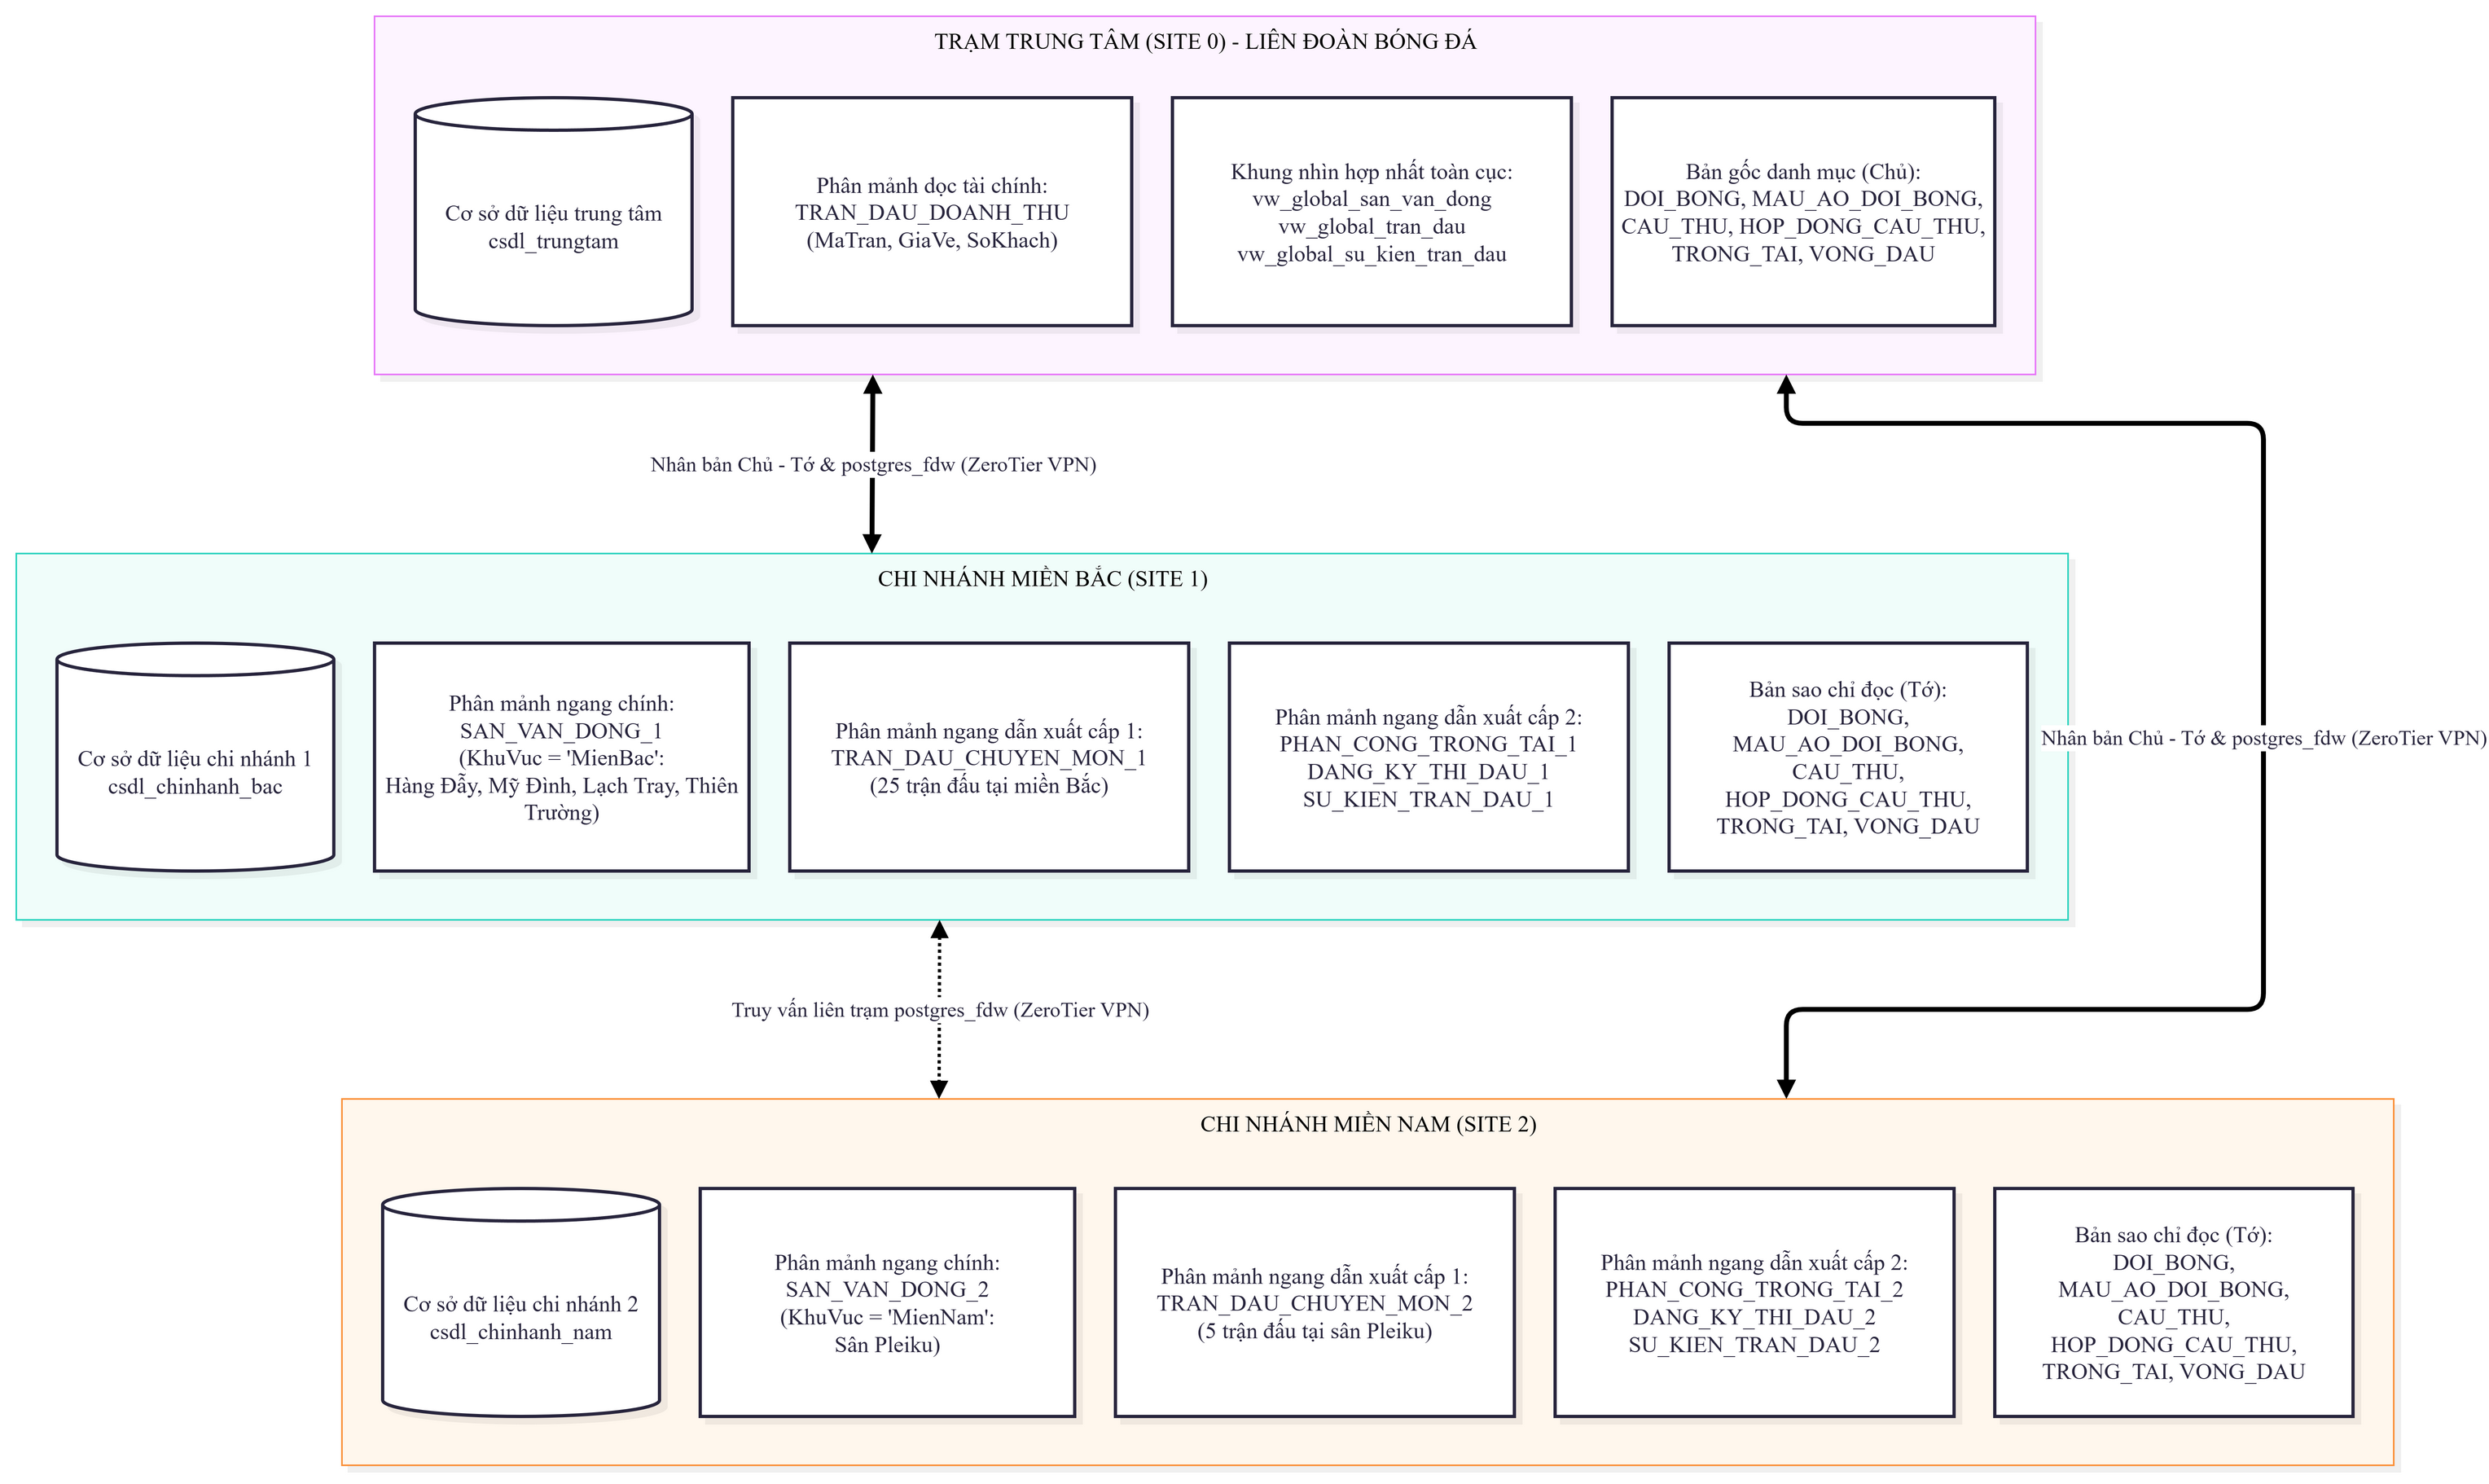
\includegraphics[angle=90, width=0.6\textheight, keepaspectratio]{Figures/DDB.png}
    \caption{Sơ đồ kiến trúc tổng quát của hệ cơ sở dữ liệu phân tán}
    \label{fig:csdl_phan_tan}
\end{figure}

\section{Triển khai kết nối liên trạm và thực nghiệm truy vấn phân tán trên PostgreSQL}

\subsection{Triển khai kết nối liên máy chủ qua mạng riêng ảo ZeroTier và tiện ích mở rộng postgres\_fdw}
Khi triển khai trên ba máy tính vật lý độc lập, các máy chủ được kết nối vào cùng một mạng riêng ảo lớp hai ZeroTier (dải địa chỉ \texttt{10.147.17.0/24}): Trạm Trung tâm (\texttt{10.147.17.10}), Chi nhánh Miền Bắc (\texttt{10.147.17.11}) và Chi nhánh Miền Nam (\texttt{10.147.17.12}). Tại máy chủ Trạm Trung tâm, tiện ích mở rộng \texttt{postgres\_fdw} được kích hoạt để ánh xạ các mảnh dữ liệu từ hai máy chủ miền về hai không gian tên \texttt{site1\_mienbac} và \texttt{site2\_miennam}:

\begin{lstlisting}[language=SQL, caption={Cấu hình kết nối liên máy chủ qua mạng ảo ZeroTier bằng postgres\_fdw}]
CREATE EXTENSION IF NOT EXISTS postgres_fdw;

CREATE SERVER srv_site1_mienbac FOREIGN DATA WRAPPER postgres_fdw
    OPTIONS (host '10.147.17.11', port '5432', dbname 'vleague_bac');
CREATE SERVER srv_site2_miennam FOREIGN DATA WRAPPER postgres_fdw
    OPTIONS (host '10.147.17.12', port '5432', dbname 'vleague_nam');

CREATE USER MAPPING FOR postgres SERVER srv_site1_mienbac
    OPTIONS (user 'postgres', password 'secret_pwd');
CREATE USER MAPPING FOR postgres SERVER srv_site2_miennam
    OPTIONS (user 'postgres', password 'secret_pwd');

IMPORT FOREIGN SCHEMA public FROM SERVER srv_site1_mienbac INTO site1_mienbac;
IMPORT FOREIGN SCHEMA public FROM SERVER srv_site2_miennam INTO site2_miennam;
\end{lstlisting}

Bên cạnh cấu hình đa máy chủ vật lý ở trên, kịch bản \texttt{06\_distributed\_simulation.sql} của đề tài đồng thời hỗ trợ khởi tạo trực tiếp ba không gian tên (\texttt{site0\_trungtam}, \texttt{site1\_mienbac}, \texttt{site2\_miennam}) trên cùng một thực thể PostgreSQL để phục vụ kiểm thử tức thì toàn bộ các phép toán đại số phân mảnh.

\subsection{Kịch bản khởi tạo phân mảnh theo đúng biểu thức đại số quan hệ}
Các câu lệnh dưới đây thực thi chính xác phân mảnh dọc bảng \texttt{TRAN\_DAU}, phân mảnh ngang nguyên thủy bảng \texttt{SAN\_VAN\_DONG} theo vị từ \texttt{KhuVuc}, và chuỗi phân mảnh ngang dẫn xuất hai cấp bằng phép bán kết nối (\texttt{WHERE EXISTS}):

\begin{lstlisting}[language=SQL, caption={Khởi tạo các phân mảnh dọc, phân mảnh ngang nguyên thủy và phân mảnh dẫn xuất}]
-- 1. Phan manh doc: TRAN_DAU_DOANH_THU luu tru doc quyen tai Site 0
CREATE TABLE site0_trungtam.TRAN_DAU_DOANH_THU (
    MaTran VARCHAR(10) PRIMARY KEY,
    GiaVe DECIMAL(12, 2) NOT NULL CHECK (GiaVe >= 0),
    SoKhach INT NOT NULL DEFAULT 0 CHECK (SoKhach >= 0)
);
INSERT INTO site0_trungtam.TRAN_DAU_DOANH_THU
SELECT MaTran, GiaVe, SoKhach FROM public.TRAN_DAU;

-- 2. Phan manh ngang nguyen thuy: SAN_VAN_DONG theo thuoc tinh KhuVuc
CREATE TABLE site1_mienbac.SAN_VAN_DONG_1 (LIKE public.SAN_VAN_DONG INCLUDING ALL);
INSERT INTO site1_mienbac.SAN_VAN_DONG_1
SELECT * FROM public.SAN_VAN_DONG WHERE KhuVuc = 'MienBac';

CREATE TABLE site2_miennam.SAN_VAN_DONG_2 (LIKE public.SAN_VAN_DONG INCLUDING ALL);
INSERT INTO site2_miennam.SAN_VAN_DONG_2
SELECT * FROM public.SAN_VAN_DONG WHERE KhuVuc = 'MienNam';

-- 3. Phan manh ngang dan xuat cap 1: TRAN_DAU_CHUYEN_MON ban ket noi voi SAN_VAN_DONG
CREATE TABLE site1_mienbac.TRAN_DAU_CHUYEN_MON_1 AS
SELECT t.MaTran, t.MaVong, t.MaDoiNha, t.MaDoiKhach, t.MaSan, t.NgayGio,
       t.BanThangNha, t.BanThangKhach, t.TheVangNha, t.TheVangKhach, t.TheDoNha, t.TheDoKhach, t.TrangThai
FROM public.TRAN_DAU t
WHERE EXISTS (SELECT 1 FROM site1_mienbac.SAN_VAN_DONG_1 s WHERE s.MaSan = t.MaSan);

CREATE TABLE site2_miennam.TRAN_DAU_CHUYEN_MON_2 AS
SELECT t.MaTran, t.MaVong, t.MaDoiNha, t.MaDoiKhach, t.MaSan, t.NgayGio,
       t.BanThangNha, t.BanThangKhach, t.TheVangNha, t.TheVangKhach, t.TheDoNha, t.TheDoKhach, t.TrangThai
FROM public.TRAN_DAU t
WHERE EXISTS (SELECT 1 FROM site2_miennam.SAN_VAN_DONG_2 s WHERE s.MaSan = t.MaSan);

-- 4. Phan manh ngang dan xuat cap 2: PHAN_CONG_TRONG_TAI, DANG_KY_THI_DAU va SU_KIEN_TRAN_DAU
-- (A) Tai Site 1 (Mien Bac): 25 tran mien Bac
CREATE TABLE site1_mienbac.PHAN_CONG_TRONG_TAI_1 (LIKE public.PHAN_CONG_TRONG_TAI INCLUDING ALL);
INSERT INTO site1_mienbac.PHAN_CONG_TRONG_TAI_1
SELECT pc.* FROM public.PHAN_CONG_TRONG_TAI pc
WHERE EXISTS (SELECT 1 FROM site1_mienbac.TRAN_DAU_CHUYEN_MON_1 t WHERE t.MaTran = pc.MaTran);

CREATE TABLE site1_mienbac.DANG_KY_THI_DAU_1 (LIKE public.DANG_KY_THI_DAU INCLUDING ALL);
INSERT INTO site1_mienbac.DANG_KY_THI_DAU_1
SELECT dk.* FROM public.DANG_KY_THI_DAU dk
WHERE EXISTS (SELECT 1 FROM site1_mienbac.TRAN_DAU_CHUYEN_MON_1 t WHERE t.MaTran = dk.MaTran);

CREATE TABLE site1_mienbac.SU_KIEN_TRAN_DAU_1 (LIKE public.SU_KIEN_TRAN_DAU INCLUDING ALL);
INSERT INTO site1_mienbac.SU_KIEN_TRAN_DAU_1
SELECT sk.* FROM public.SU_KIEN_TRAN_DAU sk
WHERE EXISTS (SELECT 1 FROM site1_mienbac.TRAN_DAU_CHUYEN_MON_1 t WHERE t.MaTran = sk.MaTran);

-- (B) Tai Site 2 (Mien Nam): 5 tran mien Nam
CREATE TABLE site2_miennam.PHAN_CONG_TRONG_TAI_2 (LIKE public.PHAN_CONG_TRONG_TAI INCLUDING ALL);
INSERT INTO site2_miennam.PHAN_CONG_TRONG_TAI_2
SELECT pc.* FROM public.PHAN_CONG_TRONG_TAI pc
WHERE EXISTS (SELECT 1 FROM site2_miennam.TRAN_DAU_CHUYEN_MON_2 t WHERE t.MaTran = pc.MaTran);

CREATE TABLE site2_miennam.DANG_KY_THI_DAU_2 (LIKE public.DANG_KY_THI_DAU INCLUDING ALL);
INSERT INTO site2_miennam.DANG_KY_THI_DAU_2
SELECT dk.* FROM public.DANG_KY_THI_DAU dk
WHERE EXISTS (SELECT 1 FROM site2_miennam.TRAN_DAU_CHUYEN_MON_2 t WHERE t.MaTran = dk.MaTran);

CREATE TABLE site2_miennam.SU_KIEN_TRAN_DAU_2 (LIKE public.SU_KIEN_TRAN_DAU INCLUDING ALL);
INSERT INTO site2_miennam.SU_KIEN_TRAN_DAU_2
SELECT sk.* FROM public.SU_KIEN_TRAN_DAU sk
WHERE EXISTS (SELECT 1 FROM site2_miennam.TRAN_DAU_CHUYEN_MON_2 t WHERE t.MaTran = sk.MaTran);
\end{lstlisting}

\subsection{Tái thiết toàn cục và tối ưu hóa truy vấn phân tán tại Trạm Trung tâm}
Tại Trạm Trung tâm, các khung nhìn toàn cục tái thiết lại quan hệ gốc bằng phép hợp (\texttt{UNION ALL}) kết hợp phép nối dọc trên khóa chính \texttt{MaTran}. Đặc biệt, đối với truy vấn thống kê Vua phá lưới toàn giải trên kiến trúc phân tán, thay vì kéo toàn bộ các bản ghi sự kiện từ hai trạm miền về Trung tâm rồi mới thực hiện phép gom nhóm, câu truy vấn được tối ưu bằng kỹ thuật \textbf{đẩy phép gom nhóm cục bộ xuống từng trạm miền}, sau đó Trạm Trung tâm chỉ cộng tổng kết quả thu gọn từ hai miền và kết nối với danh mục cầu thủ:

\begin{lstlisting}[language=SQL, caption={Tái thiết toàn cục và tối ưu hóa truy vấn Vua phá lưới phân tán}]
-- Khung nhin tai thiet toan cuc TRAN_DAU (Hop ngang + Noi doc tren MaTran)
CREATE OR REPLACE VIEW site0_trungtam.vw_global_tran_dau AS
SELECT 
    cm.MaTran, cm.MaVong, cm.MaDoiNha, cm.MaDoiKhach, cm.MaSan, cm.NgayGio,
    dt.GiaVe, dt.SoKhach,
    cm.BanThangNha, cm.BanThangKhach, cm.TheVangNha, cm.TheVangKhach, 
    cm.TheDoNha, cm.TheDoKhach, cm.TrangThai
FROM (
    SELECT * FROM site1_mienbac.TRAN_DAU_CHUYEN_MON_1
    UNION ALL
    SELECT * FROM site2_miennam.TRAN_DAU_CHUYEN_MON_2
) cm
JOIN site0_trungtam.TRAN_DAU_DOANH_THU dt ON cm.MaTran = dt.MaTran;

-- Truy van Vua pha luoi phan tan (Day phep gom nhom xuong tung Tram)
WITH BanThangPhanTan AS (
    SELECT local_agg.MaCauThu, SUM(local_agg.SoBan) AS TongBanThang
    FROM (
        SELECT sk1.MaCauThu, COUNT(*) AS SoBan
        FROM site1_mienbac.SU_KIEN_TRAN_DAU_1 sk1
        WHERE sk1.LoaiSuKien = 'BanThang' GROUP BY sk1.MaCauThu
        UNION ALL
        SELECT sk2.MaCauThu, COUNT(*) AS SoBan
        FROM site2_miennam.SU_KIEN_TRAN_DAU_2 sk2
        WHERE sk2.LoaiSuKien = 'BanThang' GROUP BY sk2.MaCauThu
    ) local_agg GROUP BY local_agg.MaCauThu
),
DoiBongHienTai AS (
    SELECT DISTINCT ON (hd.MaCauThu) hd.MaCauThu, db.TenDoi
    FROM site0_trungtam.HOP_DONG_CAU_THU hd
    JOIN site0_trungtam.DOI_BONG db ON hd.MaDoiHienTai = db.MaDoi
    WHERE hd.TrangThai IN ('ChinhThuc', 'ChoMuon')
    ORDER BY hd.MaCauThu, hd.NgayBatDau DESC
)
SELECT ROW_NUMBER() OVER (ORDER BY b.TongBanThang DESC, ct.HoTen ASC) AS XepHang,
       ct.MaCauThu, ct.HoTen, COALESCE(d.TenDoi, 'Tu do') AS TenDoiHienTai, b.TongBanThang
FROM BanThangPhanTan b
JOIN site0_trungtam.CAU_THU ct ON b.MaCauThu = ct.MaCauThu
LEFT JOIN DoiBongHienTai d ON b.MaCauThu = d.MaCauThu
ORDER BY b.TongBanThang DESC, ct.HoTen ASC LIMIT 10;
\end{lstlisting}

Kết quả thực nghiệm xác nhận Chi nhánh Miền Bắc quản lý 4 sân vận động và 25 trận đấu, Chi nhánh Miền Nam quản lý 1 sân vận động và 5 trận đấu, và khung nhìn toàn cục tại Trạm Trung tâm tái thiết chính xác 30 trận đấu cùng đầy đủ thông tin doanh thu bán vé và bảng xếp hạng Vua phá lưới trùng khớp $100\%$ với cơ sở dữ liệu tập trung. Mô hình bảo đảm trọn vẹn tính trong suốt phân mảnh, tính trong suốt vị trí và tính trong suốt nhân bản đối với các ứng dụng khai thác.

% \include{Chapters/05-GiaoDienVaThuNghiem}

% Tài liệu tham khảo
\printbibliography

% Trang bìa sau
\ifthenelse{\equal{\getLanguage}{portuguese}}{%
    \pdfbookmark[0]{Contra Capa}{contracapa} % Add entry to PDF
}{%
    \pdfbookmark[0]{Back Page}{backpage} % Add entry to PDF
}


\clearpage
\null
\thispagestyle{empty}

\newcommand\BackgroundPicBackPage{%
    \put(0,0){%
    \parbox[b][\paperheight]{\paperwidth}{%
    \vfill
    \centering
    
\includegraphics[width=\paperwidth,height=\paperheight,keepaspectratio]{Figures/Theme/Back-Page-BG.pdf}%
    \vfill
}}}
\AddToShipoutPictureBG*{\BackgroundPicBackPage}

\newgeometry{margin=1.98cm, top=1.47cm, bottom=1.47cm}
\noindent\clearpage
\restoregeometry

\end{document}
